\chapter{Apparatus}
\label{Chap_Apparatus}

% epigraph (done 2021-8-24 09:23:49)
\setlength{\unitlength}{1pt}
\setlength{\epigraphwidth}{10.5cm}
\epigraph{工欲善其事,必先利其器。\\ A craftsman must sharpen his tools to do his job.}{--- Confucius\\ \textit{The Analects (5th century BC)}}

% introduction (done 2021-9-16 16:08:33)
This chapter describes the Na-Rb machine and the upgrades we made for our droplet experiment. As most of the setup has been described by the previous thesis \cite{WangFudong2016Soau,LiXiaoke2015Chsd}, we only shortly make a summary in Sec. \ref{sec:machine} for the completeness of this chapter. In Sec. \ref{sec:image}, we turn to the image system upgrades for measuring the droplet sample with several $\mu$m sizes. We design a 15$\times$ magnification image system with a resolution of 2 $\mu$m. Besides, we upgraded the mechanical part onto an electro-translation stage, which can follow the ToF of the free-falling sample without worsening the image resolution. We detailedly describe the high-magnetic field in-situ image scheme for subtracting the sample's density profile reliable. To control more cameras from different manufacturers, I built a multi-camera control platform with image processing called CAMIMA. We will introduce it in Sec. \ref{sec:camima} as a manual for future using and upgrading. Finally, we discuss several improvements such as fast-coil for fast controlling magnetic field (Sec. \ref{sec:fastcoil}), magnetic field gradient compensation (Sec. \ref{subsec:gradientcompen}) and coil antennas for increasing the Rabi frequency of Rb (Na) micro-wave transition (Sec. \ref{subsec:FWLA}).

\section{Overview: Na-Rb machine I}
\label{sec:machine}

% goal of this Na-Rb machine (done 2021-8-24 10:28:43)
A cold atom machine capable of producing reproducible samples with stable atomic conditions is indispensable for the following experiments. So, even though the Na-Rb machine in our laboratory has been running for longer than eight years, many aspects still need to improve to make the sample condition more stable. \cite{LiLintao2021} describes many efforts we made: optimization of the micro-wave evaporation procedure for Rb sympathies cooling of Na; a new ultra-stable magnetic field servo system for achieving hundred-Gauss with only two mG level fluctuation. Besides stability, producing more atoms is another goal for many experiments because there are always various types of loss during preparing the atomic (or molecular) samples. More numbers of final sample can make detection easier and offer more opportunities to study new physics. In the droplet experiment \cite{guo2021leehuangyang}, if we produce a sample with ten times more numbers (i.e. $10^6$ for each species), we can study more properties of the bulk sample, such as flat-top density profile \cite{petrov2015}, the surface excitation modes \cite{petrov2015} and achieving a longer lifetime.

% overall system (done 2021-9-16 17:18:52)
\begin{figure}[htb]
\begin{center}
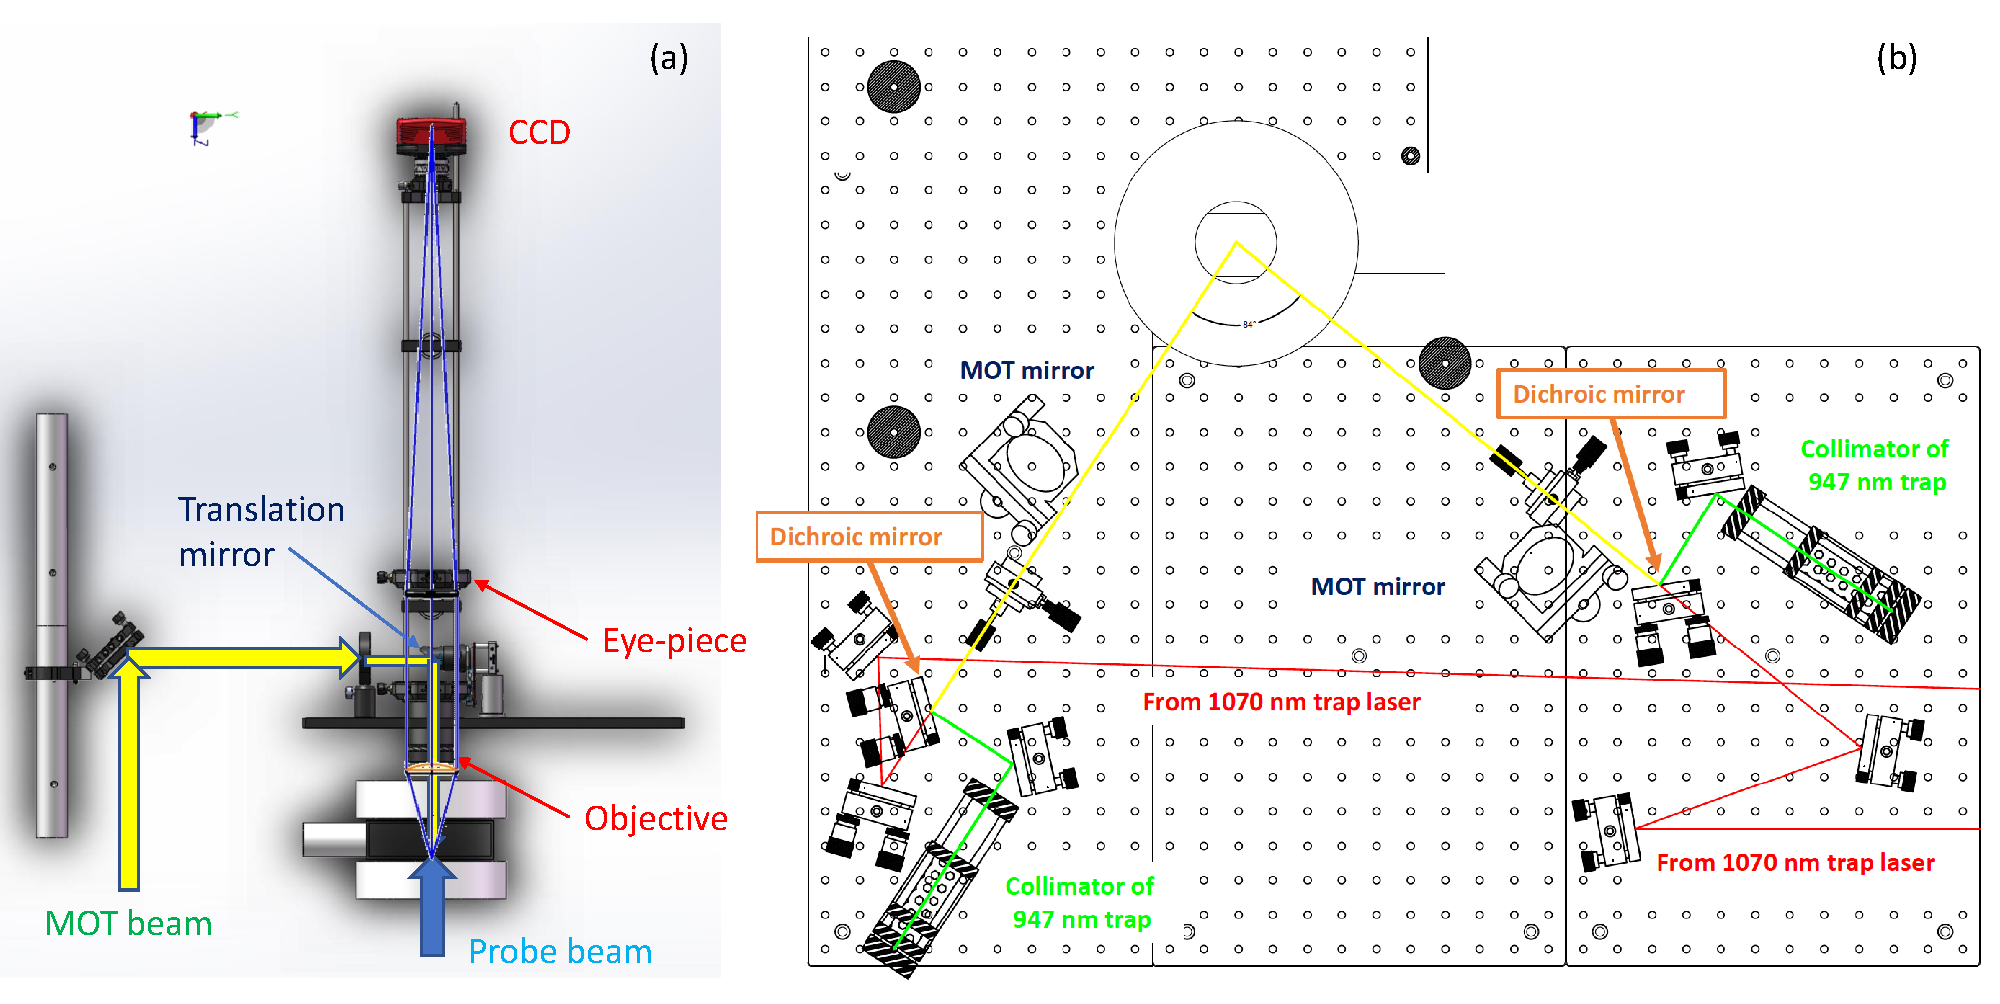
\includegraphics[width = \linewidth]{figures/Apparatus_overall.pdf}
\end{center}
\caption[Front and top view of overall Na-Rb machine]{(a) shows the Front view of the Na-Rb machine. The up-down image(pumping) shares the same optical path with MOT laser. After MOT loading, we switch the mirror cart away to leave path for up-down image. (b) shows the optical trap laser layout as a top view. Image is taken from \cite{LiLintao2021}}
\label{Apparatus_overall}
\end{figure}

\subsection{Producing Na-Rb Bose-Einstein condensate mixtures}

% Dispenser, LIAD method for loading (done 2021-8-25 11:00:14)
Our experiment starts from Na and Rb dispensers. We fire the Rb dispenser every day with a relatively low current of 1.9 A (temperature of less than 500 K). Na dispenser fires only once a month, however, with a relatively high current (3.5 A) and temperature (600 K). The temperature and current conversion chart is shown in Fig, \ref{Apparatus_dispen}. The reason for not firing the Na dispenser at a low current is that the temperature for turning on the Na dispenser (Na starts to spray out) is still too high and breaks the vacuum. Since we use a single chamber design, we have to make the trade-off between the loading rate of MOT and the vacuum condition. Thanks to the light-induced atomic desorption (LIAD) method, we can increase the atoms flux (for both Rb and Na) for MOT loading by turning UV on at the beginning of each shot. Of course, this will degrade the vacuum condition in the chamber, however, after MOT loading, we turn off the UV, and the atom can be absorbed again by the chamber and then the vacuum recovers. The typical lifetime of Rb in the quadruple trap (QT) is 30 s level, and Optical-trap (OT) lifetime is about 20 s. 

% dispenser (done 2021-8-25 10:24:28)
\begin{figure}[htb]
\begin{center}
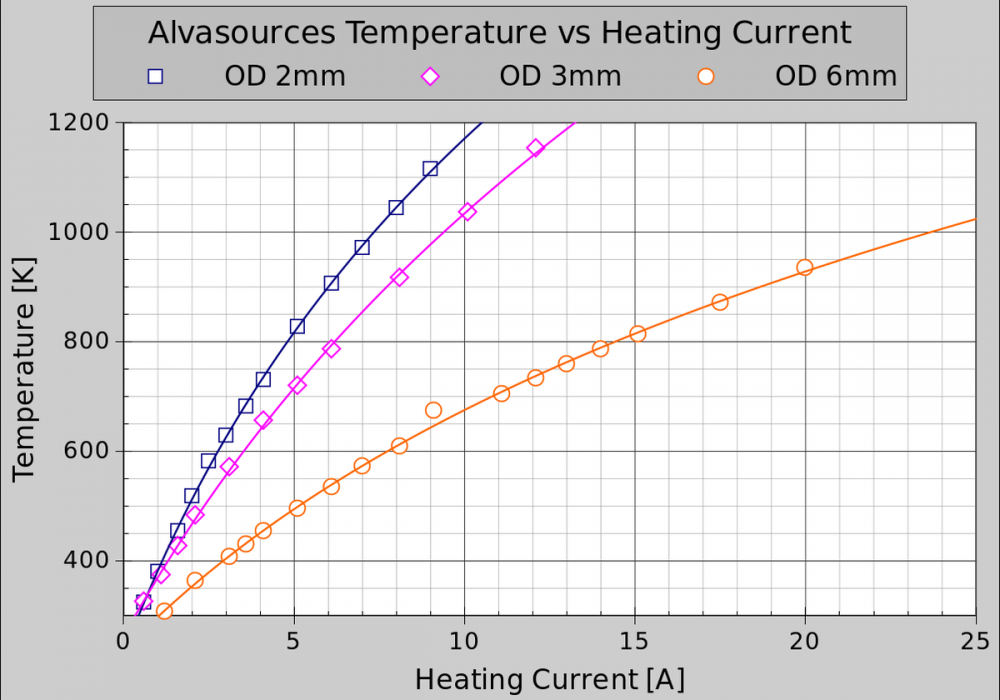
\includegraphics[width = 0.7\linewidth]{figures/Apparatus_dispen.png}
\end{center}
\caption[Temperature-current relationship of dispenser (Image from \href{https://alfavakuo.eu/products/mvs/}{alfavakuo})]{Temperature-current relationship of dispenser (Image from \href{https://alfavakuo.eu/products/mvs/}{alfavakuo}). The dispenser of Na and Rb are both with diameter of 3 mm.}
\label{Apparatus_dispen}
\end{figure}

% CMOT, molasses (done 2021-8-26 14:28:05)
After atoms gradually accumulating within 30 seconds, Na and Rb MOT finally achieves saturation. To avoid collision between Rb and Na that induces an inelastic process, we use a resonance light to push the Rb MOT aside to avoid overlapping Na and Rb. That dual MOT typically can capture $10^{9}$ Rb and $1.5 \times 10^{6}$ Na. To increase its density, we apply a compress-MOT (CMOT) process, which increases the restoring force by far detuning the MOT laser\footnote{in our experiment, we do not increase the magnetic gradient.}. To further increase the phase space density (PSD) of the sample, a molasses process is implemented to cool the sample further. Finally, we load the sample into QT with both species in $\ket{F=1,m_F=-1}$ state.

% In QT and QT evaporation and hybrid trap (done 2021-8-26 14:53:38)
A pair of the anti-Helmholtz coil generates the Quadrupole trap (QT). At the beginning of the time sequence, the magnetic gradient is ramped up to 160 G/cm, served as a conservation trap for capture all atoms from the precooling stage. Then, we do the evaporation cooling for Rb which using a MW to pump atoms from $\ket{F=1,m_F=-1}$ to $\ket{F=2,m_F=0}$. Due to the anti-trapping of $\ket{F=2,m_F=0}$ state, we can remove the high-temperature atoms away from the trap to decrease the overall sample temperature. Na atoms are sympathetically cooled by Rb. Due to Majorana loss bringing anti-evaporation effect, we add a single beam optical trap to shift the minimum position of the whole potential away from the QT centre. This works at the first evaporation stage and helps us obtain a sample with 20 $\mu$K temperature. After that, we adiabatically lower down the QT to 26 G/cm for avoiding severe Majorana loss further. After the MW sweeping to 6833 MHz, we finally achieve a mixture sample with temperature around several $\mu$K. This allows us to load them to an Optical dipole trap to do further cooling and experiment. More details about this hybrid trap can be found in this note of our lab \cite{xiong2013production}.

% In OT and OT evaporation (done 2021-8-26 15:09:24)
Optical trap evaporation is achieved by forcibly reducing the light intensity. In the later stage, the atomic density becomes lower due to the weakening of confinement, which reduces the collision rate, so a slower evaporation rate is required. As a result, the optical trap evaporation is relatively inefficient. Using 1070 crossed OT in our experiment, we typically spend 3 s to obtain a two-species BEC. For a one-dimensional optical trap, the evaporation time requires even longer and may take 5-10s. Therefore, we generally obtain BEC in the 1070 XOT first and then transfer it to other types of optical traps for experiments. Of course, the transfer process will inevitably bring excitation, so it is crucial to deceive an adiabatic process or wait a long enough time for reaching the ground state.

% state preparation (done 2021-8-26 20:11:43)
Since we need the Feshbach resonance between Na and Rb both in  $\ket{F=1,m_F=1}$ state, we need transfer atoms from $\ket{F=1,m_F=-1}$ to the target state. The easiest and most robust way is the adiabatic-rapid passage (ARP). By applying an RF(or MW) field to couple the initial and target state, we can detune its detuning from the blue (red) side to the red (blue) side. Following the dressed state, atoms start from $\ket{F=1,m_F=-1}$ however end with $\ket{F=1,m_F=1}$. This procedure needs enough adiabaticity, which is time-consuming; however, it is robust from the system's power fluctuation and time precision. We carry out the transition under a low magnetic field, which enables us couple the $\ket{F=1,m_F=-1}$ state to $\ket{F=1,m_F=0}$ and then to $\ket{F=1,m_F=1}$. For latter experiments that need $\ket{F=1,m_F=0}$, we can apply a relatively high magnetic field to decouple these two transitions. More details can be found in the previous thesis \cite{WangFudong2016Soau,LiXiaoke2015Chsd,LiLintao2021}.

% 1070 and 946 ODT (done 2021-8-26 15:24:14)
\begin{figure}[htb]
\begin{center}
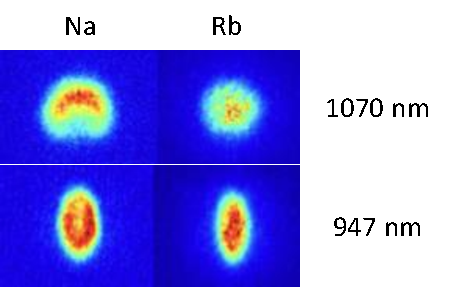
\includegraphics[width = 0.6\linewidth]{figures/OT_1070-946.pdf}
\end{center}
\caption[Na and Rb samples in 946 and 1070 nm ODT (image from \cite{LiLintao2021})]{Na and Rb samples in 946 and 1070 nm ODT (image from \cite{LiLintao2021}). Due to gravitational sag difference, Na in 1070 ODT is buoyant above Rb. In 946 nm ODT, Rb stays at the centre of Na, showing the sag difference's excellent compensation.}
\label{OT_1070-946}
\end{figure}

% BEC mixture (done 2021-8-26 16:49:43)
In our experiment, Na has a relatively large interaction strength $g_{Na}$ (even its scattering length is smaller than Rb, its mass three times smaller than Rb.), so at the beginning of OT evaporation, it is Na sympathetically cooling Rb. However, typically Na becomes BEC before Rb does because of a higher transition temperature, which is mainly due to the higher trap frequency of Na in the 1070 nm ODT. After that, the evaporation is mainly for the Rb sample, and we can achieve a two-species BEC with an almost balanced number at the final. This number ratio actually can be tuned by changing the evaporation ending in QT. For the double BEC sample in ODT, Na is immiscible with Rb in the case of a low magnetic field. Thus, Na shows a crescent shape which is because of the gravitational sag difference of two samples (shown in Fig. \ref{OT_1070-946}). In order to obtain a relatively pure BEC sample, we lower down the optical trap to a relatively shallow level, such as about 80 Hz for Na in 1070 ODT. We check the purity of the BEC sample by observing the BEC sample without any thermal part for whatever ToF. Then, we say that the sample is pure enough. However, to characterize the temperature of this sample, correspondingly the BEC fraction, is typically hard, which is beyond the range of this thesis.

% number ratio control (done 2021-8-26 17:54:39)
In many experiments, we need to control the number ratio of Na and Rb. The typical method is to adjust the optical trap's relative position to the QT's zero-point. By modifying this distance, we can determine the atomic number of Rb after the QT evaporation. Rb will be less evaporated and more Rb atoms remain for a longer distance, vice versa. Because the Na number is much less than Rb, with sympathetically cooled, the Na number mainly unchanges. However, the temperature will be the same as Rb. Subsequently, the evaporation of loading into OT is dominated by Na, as mentioned before. Therefore, the number ratio of Na and Rb can be manipulated by changing the number of the remaining Rb after QT evaporation.

% 946 trap (done 2021-8-27 10:40:15)
As described in \cite{LiLintao2021}, we build an optical trap with magic wavelength, which offers the same trap frequency for both Na and Rb. As shown in Fig. \ref{OT_1070-946}, Rb stays at the centre of Na. We can benefit a lot from this wavelength, such as increasing the overlap between Na and Rb and consequently increasing the Feshbach molecule's conversion rate or enhancing the signal of the polaron experiment. Our droplet experiment uses this sag-difference-free trap to achieve better overlap and form droplets with lower density and longer lifetime, which will be discussed in Chap. \ref{Chap_droplet}.

\subsection{Producing Na-Rb Feshbach molecules}
% motivation (done 2021-8-26 18:49:35)
In our laboratory, the original intention of producing Feshbach molecules is to make the ground state molecule of NaRb further. After successfully making the ground state molecule \cite{PhysRevLett.116.205303}, the mission of this machine becomes the study of heteronuclear mixture BEC. The core ingredient of research on this set-up consequently involves adjusting inter-particle interaction through the Feshbach resonance. Many interesting physics problems can be studied, such as Effimov state, polaron, spinor. Then the essential parameter is the FR parameter, i.e. how the scattering length of the inter-species changes with the magnetic field. The detailed calibration and calculation will be demonstrated in Chap. \ref{Chap_Feshbach}. We note that the scattering properties near resonance will be most affected by the shallowest bound state, so the precision measurement of the bound state will give accurate scattering properties in turn. Therefore, we need to synthesize FR molecules and study their properties.

% method (done 2021-8-27 10:40:51)
Our experiment starts from an optically trapped ultracold mixture of $^{23}$Na and $^{87}$Rb atoms, both in their lowest hyperfine state $\ket{F = 1, m_F = 1}$~\cite{wang2013observation,wang2015formation,jia2020}. Magnetoassociation starts from an initial magnetic field of 350 G, just above the FR at $B_0 = 347.64$ G. The magnetic field is ramped down across the resonance to form FMs, and then to 335.6 G. At this field, the FMs have a nearly zero magnetic dipole moment; this allows us to remove the residual atoms with a short and strong magnetic field gradient without losing molecules. Afterwards, the magnetic field is ramped up to a range of target values below $B_0$ for further experiments. Following this procedure, we can routinely obtain a pure sample of $^{23}$Na$^{87}$Rb FMs with a typical temperature of 300 nK and a trap lifetime of more than 30 ms. This short lifetime is due to near-resonance photon scattering by the 947 nm optical trap light~\cite{Guo2017,jia2020}, which is provided by a home-built diode laser system. In another experiment on $^{23}$Na$^{87}$Rb, in which a single-frequency 1064 nm laser is used as the optical trap light, FM lifetimes greater than 100 ms have been observed~\cite{Wang2019,guo2021leehuangyang}. Nevertheless, the current lifetime is more than enough for the present work, as we need only 10 ms for magnetic field stabilization and less than 1 ms for dissociation.

\section{Image system upgrades}
\label{sec:image}

% motivation: why upgrade image system (done 2021-8-27 11:04:57)
The previous image system is composed of an f=100mm (\#49360-INK) and f=300 mm (\#49368-INK) pair from Edmund optics, which can support a resolution of about 3 $\mu$m (N.A.=0.13) as shown in Fig. \ref{old_image}. This imaging system is built with discrete elements, which cannot move
as a whole. Thus, it is only proper for imaging for a small region; otherwise, both spherical aberration and coma shows up if moving only the camera or the lens set. We need to do the ToF for samples for the droplet experiment, and the displacement reaches about 2 mm. If we change the camera position, the resolution for imaging sample with large displacement, i.e. at the edge of field-of-view, will be degraded. So, we improved our resolution by two means: First, we increase the imaging system's resolution by using a long working distance objective; secondly, we build a whole block by mounting all optical elements and cameras onto an electric translation stage. In the rest of this section, we discuss the absorption image method for a dense atomic cloud, introduce a high-magnetic-field image scheme, and discuss the number calibration method.

% old imaging system (done 2021-9-16 17:21:13)
\begin{figure}[htbp]
\begin{center}
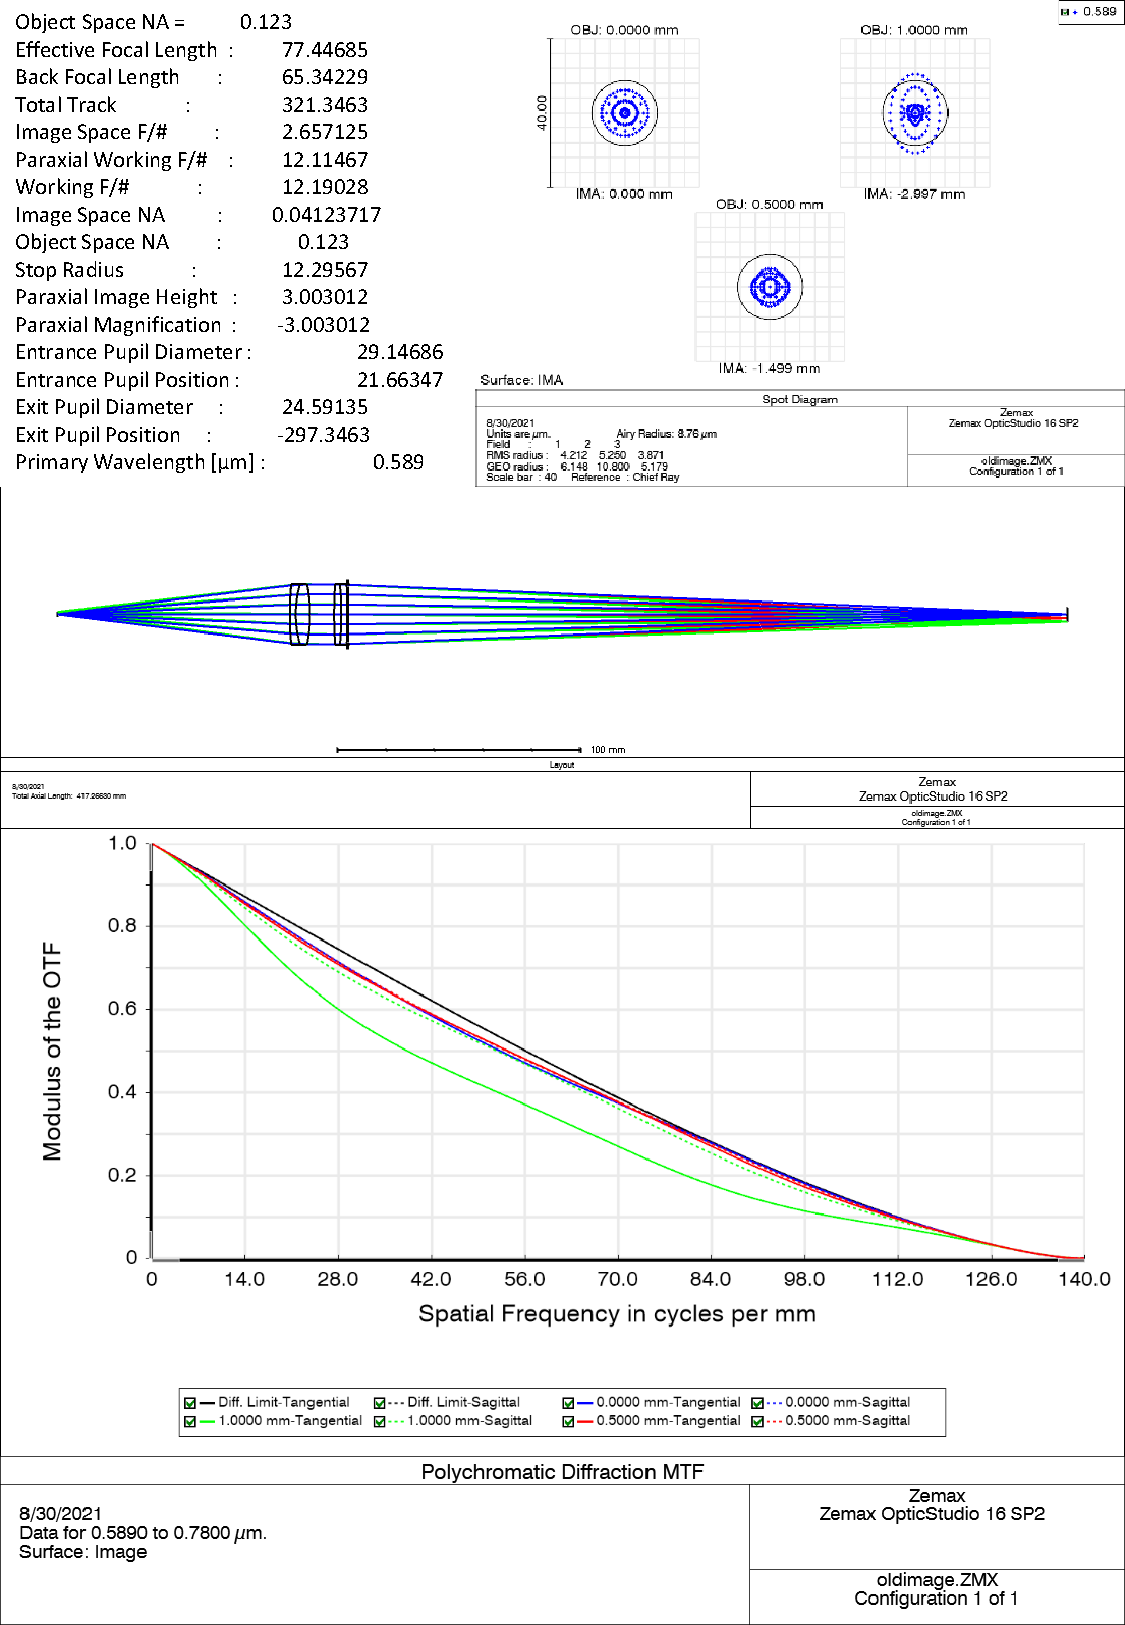
\includegraphics[width = \linewidth]{figures/old image.pdf}
\end{center}
\caption[3x image system simulation by Zemax]{3x image system simulation by Zemax. From the spot diagram and MTF calculation, we can read out a large field-of-view of this system.}
\label{old_image}
\end{figure}

\subsection{High resolution image system}

% optical design (done 2021-8-27 14:44:36)
The characteristic length for a droplet is typical of several $\mu$m, as shown in Sec. \ref{Chap_droplet}. In order to resolve this tiny sample, we need a better imaging system with resolution reaching $\mu$m level. The old imaging system with an f=100mm objective is not enough since its N.A. is 0.13 with an airy radius of about 4 $\mu$m. So, we use an objective with a shorter focal length to increase N.A. The most convenient way is using a microscope with a long working distance. So, we choose a 10X Mitutoyo plan-apo infinity-corrected Long-WD objective with an effective focal length of 20 mm. Its working distance reaches 34 mm, enough for our application without blocking any optical path, such as MOT or optical trap. We can use the same eyepiece (Edmund \#49368) with f=300 mm and directly image the atom onto the camera thanks to the infinity-correction property. 

% mechanical design (done 2021-8-27 15:09:52)
As shown in Fig. \ref{image_system}, We use the cage system from Thorlabs to build the main body of the imaging system. A $45^\circ$ mirror reflects the probe beam in the vertical direction. This avoids the diffraction light from optical dipole trap scattering to CCD and affects the image quality. The dichromatic mirror can be tuned to ensure the Na image is at the centre of Na CCD. Moreover, we add a ring adjuster for Rb CCD to fine-tune its position. This is mainly for focusing on both Na and Rb. Because there always be a chromatic shift for two different wavelengths (589 nm for Na and 780 nm for Rb). So, when focusing on the system, we first focus the Na by move the set-up as a whole, i.e. move the objective on focus to the atom. Then, we tune the ring adjuster to focus Rb onto the camera. One mistake is that we choose an adjuster too fine (4 mm for ten turns), so the adjustment procedure typical take a long time. As mentioned before, the whole system is mounted onto an electric translation stage controlled by an Arduino. Code and control can be found in Lintao's thesis \cite{LiLintao2021}.

% High-field image scheme (done 2021-8-27 15:12:52)
\begin{figure}[htb]
\begin{center}
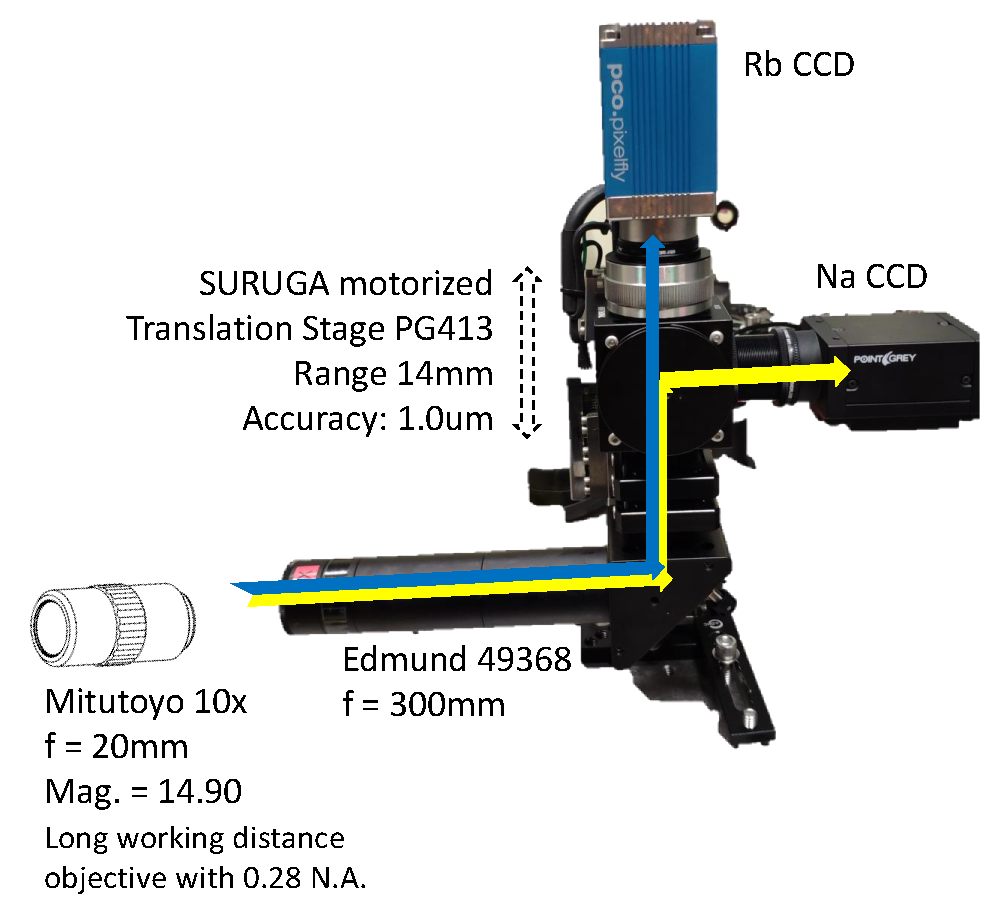
\includegraphics[width = 0.8\linewidth]{figures/image_system.pdf}
\end{center}
\caption[New compact imaging system]{New compact imaging system. The whole set-up is mounted on a electric translation stage from SURUGA. The objective can be switched between a Mitutoyo 10x microscope and a typical f=100 mm achromatic lens. Then follows a f=300 mm eyepiece for focusing. A dichromatic mirror splits Rb and Na probe into two CCDs.}
\label{image_system}
\end{figure}

% cell wall effect (done 2021-8-27 15:35:56)
Even though we use a powerful objective with an Airy radius of 1 $\mu$m, there exists a critical issue that the cell wall is 3 mm thick. So, we need to check the imaging system's performance with this 3 mm window before the objective. We did not do any correction for this glass wall because our primary goal is to increase the magnification. Even the resolution only increase twice will be enough for observing droplet signals. The 3 mm window will decrease the resolution\footnote{A tutorial for standard object correction ring can be found \href{ http://www.mvi-inc.com/wp-content/uploads/Use-of-the-Correction-Ring-on-the-Objective.pdf}{here}. Moreover, the effects of thick glass on an imaging system can be found on \href{https://www.thorlabs.com/newgrouppage9.cfm?objectgroup_id=9895&pn=TL2X-SAP}{Thorlabs} under the tag of correction collar}. Since when the focused beam goes through the glass wall, light with a different angle will bend by different amplitude and finally, they cannot converge to a single point as without the glass. This effect is severe when the N.A. goes higher.

% resolution test (done 2021-9-16 19:04:44)
\begin{figure}[htb]
\begin{center}
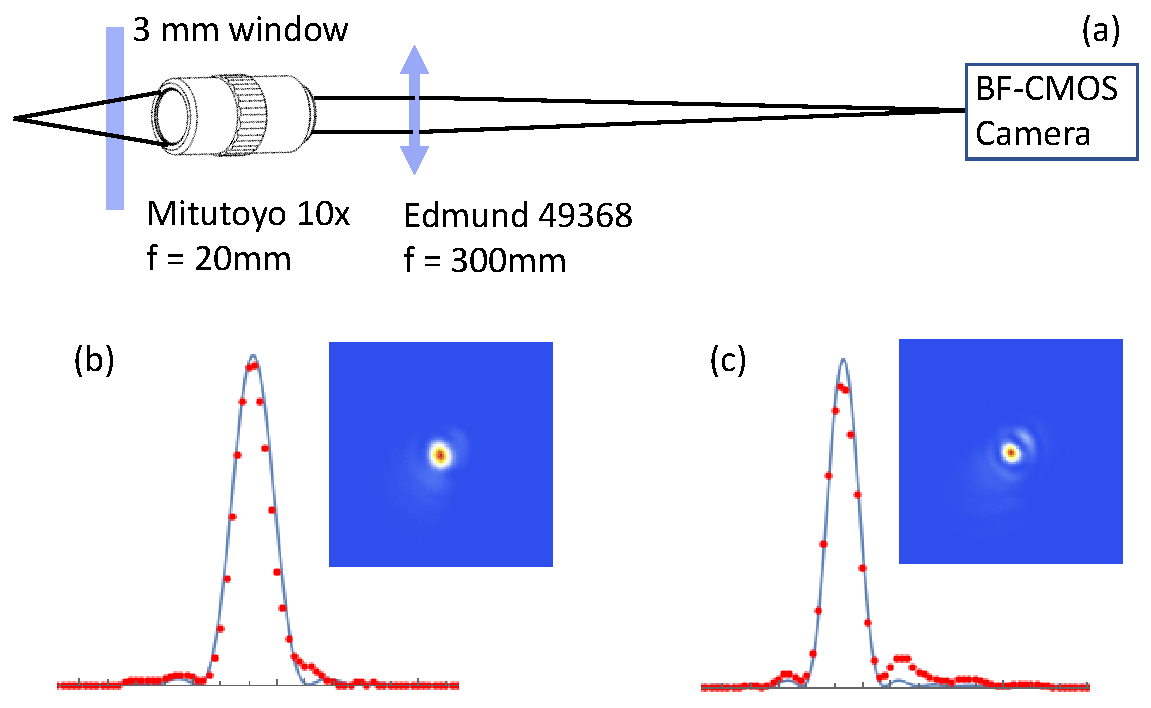
\includegraphics[width = 0.9\linewidth]{figures/Apparatus_image-reso.pdf}
\end{center}
\caption[Image resolution test of 15x image system]{Image resolution test of 15x image system. (a) shows the test method. a 2 $\mu$m pin-hole is used as target. Image is taken be a pixel-size 3.45 $\mu$m Blackfly CMOS camera. (b) and (c) shows the airy disk we measured for Rb and Na.}
\label{image_reso}
\end{figure}

% test resolution (done 2021-8-27 15:49:18)
Before putting it online, we first test its resolution offline with a USAF1951 target and 2 $\mu$m pinhole. Here, we show the measured Airy disk in Fig. \ref{image_reso}. By simply fitting the pattern with the Airy function, we get the resolution for Na(Rb) is 1.7(2.3) $\mu$m. So we now have a high resolution and commercial and cheap image system. 

% Translation stage (done 2021-8-27 16:44:06)
Because we will do ToF measurement for several tens of ms, i.e. about 2 mm away from the centre of view-of-field, spherical aberration and coma can worsen the image quality. This can be shown by Zemax by a tilted angle of input light (Fig. \ref{image_reso}). We use a high magnification imaging system with a short focal length of 20 mm. This makes its field-of-view very small. So, we need to move the whole imaging system along with the atomic sample. So, we build the imaging system very compact and mount it onto a translation stage controlled by a computer. The translation stage is mounted vertically with a step resolution of 1 $\mu$m. We use an Arduino board to control the driver. Finally, we can change the position of our image system at will shot by shot. To avoid the movement changing affecting the EM field around the cell, we make each movement at the interval of two shots.

\subsection{High magnetic field absorption image}
\label{subsec:high_mag_absop_image}

% goal (done 2021-8-27 16:47:15)
To probe the droplet without distortion, we need the imaging scheme reliable, which means the method can recover the density profile of the sample as accurate as possible. Since a typical droplet sample has OD above 50 for Rb and 10 for Na, a typical absorption image method cannot be used directly, which is because the absorption image's SNR is limited when the sample OD is too high. As plotted in Fig. \ref{SNR_OD}, weak probe intensity (less than one saturation intensity) can only support OD smaller than 3 \cite{guo2021SNR}. Increasing the probe intensity to achieve the saturation absorption image can increase the threshold of OD to probe. However, higher intensity could cause several other problems: first, calibration could be hard to do or cause a significant error because the nonlinear response of the absorption. second, for a high density sample the re-scattering problem could introduce the effect beyond the aforementioned theory. So, we conceive a partial pumping method and a high-magnetic field absorption imaging scheme for the high-OD samples.

% SNR of absorption image as a function of OD (done 2021-9-18 15:21:00)
\begin{figure}[htb]
\begin{center}
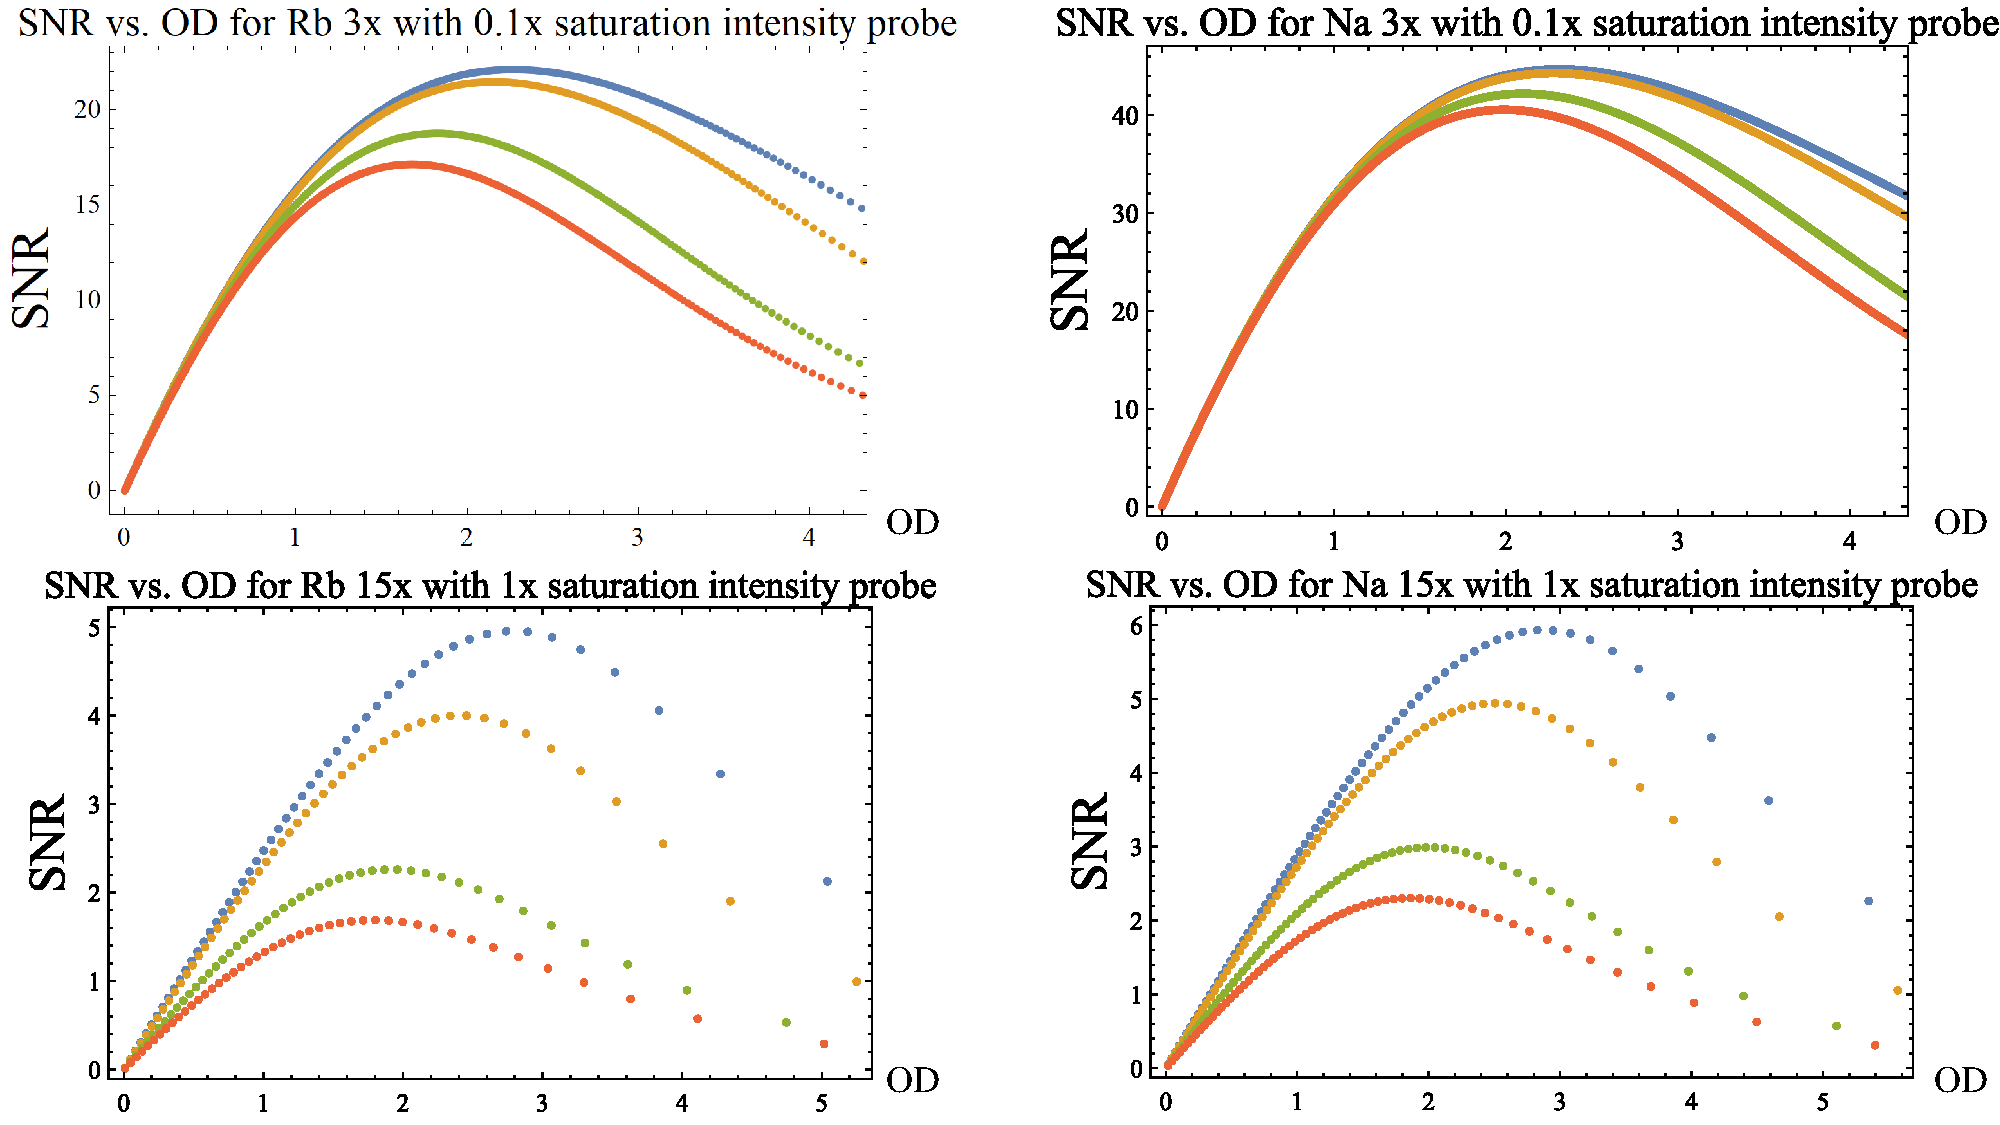
\includegraphics[width = \linewidth]{figures/Apparatus_AI_SNR.pdf}
\end{center}
\caption[SNR of absorption image as a function of OD]{SNR of absorption image as a function of OD. Above two panels are our 3x image system, and Lower two panels are our 15x image system. Blue dots for PCO-sCMOS camera; yellow dots for BFS-PGE-31S4; green dots for PCO double-image camera; orange dots for Pointgrey 51S5.}
\label{SNR_OD}
\end{figure}

% image scheme (done 2021-8-27 17:47:45)
Thus, we first decrease the sample's density; however, we keep its profile unchanged. Then, we apply the typical absorption image. This is what we called the partial pumping method for absorption image. A typical way to pump a small portion of the sample to the image transition is by MW or light. As shown in Fig. \ref{image_system}, our sample is at $\ket{F=1,mF=1}$ state, which is non reacting with the absorption light. Then, we use a pumping laser to pump atoms to exited state $\ket{m_J=1/2,m_I=3/2}$; then, with spontaneous radiation, atoms accumulate onto $\ket{F=2,m_F=2}$ state. Finally, we use the cycling transition from this state to $\ket{m_J=3/2,m_I=3/2}$ state to do the absorption image. Here the pumping can also be done by the MW pulse. However, our original MW had a Rabi freq less than 10 kHz, which could consume 100 $\mu$s or even longer apply a $\pi$ pulse. This would make the sample's shape changed a lot when we probe it by the image light. We will get back to this point when we discuss our upgrades of the Full-wave loop-antenna in Sec. \ref{subsec:FWLA}. 

% High-field image scheme (done 2021-8-27 16:52:34)
\begin{figure}[htbp]
\begin{center}
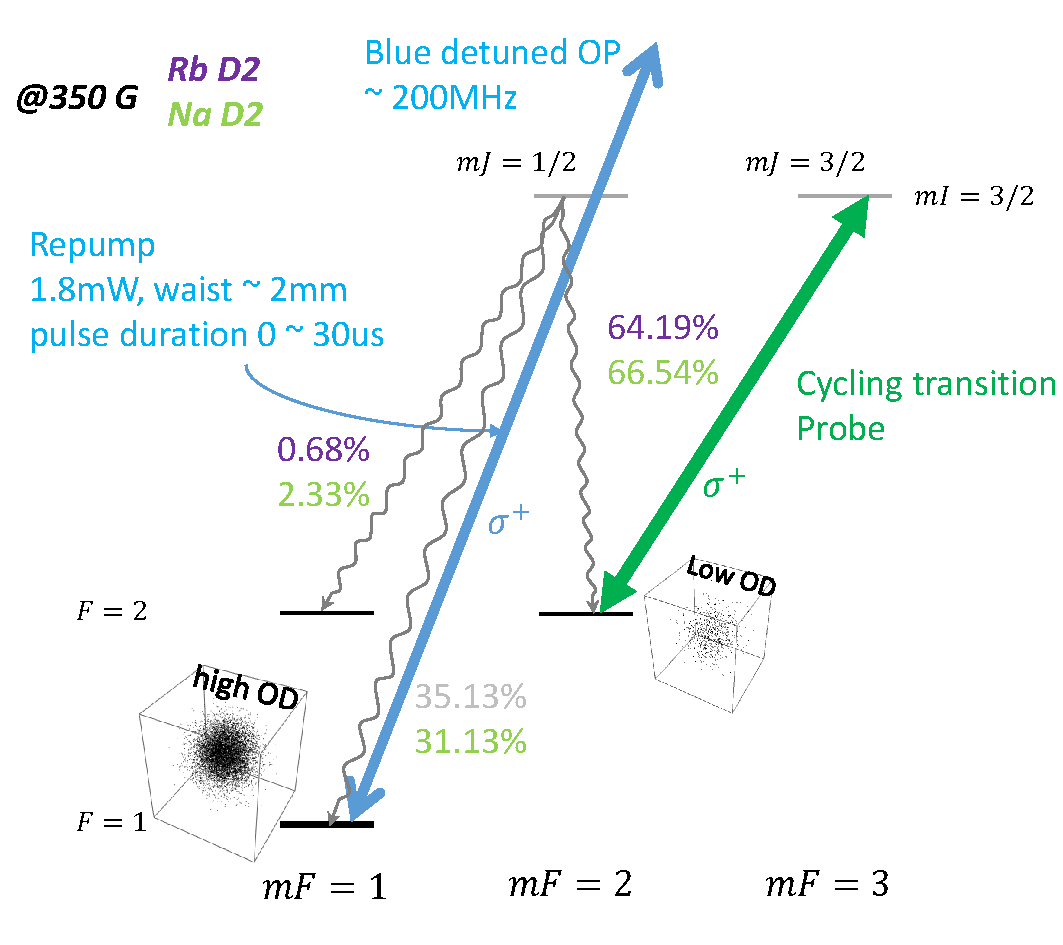
\includegraphics[width = 0.8\linewidth]{figures/High-field image scheme.pdf}
\end{center}
\caption[image scheme for Na(Rb) $\ket{F=1,m_F=1}$ state under 350 G magnetic field]{image scheme for Na(Rb) $\ket{F=1,m_F=1}$ state under 350 G magnetic field. The ground states are labelled with F and $m_F$; the excited states are labelled with $m_J$ and $m_I$. The imaging procedure is divided into two steps: first, pumping atoms from $\ket{F=1,m_F=1}$ to $\ket{m_J=1/2,m_I=3/2}$. After atoms accumulating to $\ket{F=2,m_F=2}$ state, we drive the cycling transition for absorption image. By blue detuning about 200 MHz of the pumping light, we can control the pumping ratio to control the OD for the image transition.}
\label{High-field image sheme}
\end{figure}

% partial pumping (done 2021-8-27 18:02:39)
So, we choose the pumping laser instead of tuned to on resonance, and we make it large detuned away from the transition and make its intensity high. This method ensures the whole sample feel around the same intensity because large detuning and intensity make the atoms only absorb a tiny portion of the light. Even for a very dense sample, the unevenness of the saturation effect can be avoided. As plotted in Fig. \ref{High-field image sheme}, Na partial pumping a small portion of the sample to $\ket{F=2,m_F=2}$ state, which then can be detected directly. The pumping ratio can be controlled by the duration of the pumping laser. As shown in Fig. \ref{partial pumping}, the OD of pumped Na atoms as a function of the pumping duration is plotted. We can see that we have an almost linear pumping speed for the first several tens of us, and after 50 $\mu$s we have a saturation effect. This saturation effect is used to calibrate latterly. For our experiment, to decrease the OD to less than 3, we typical using a detuning 200-300 MHz and pumping only several $\mu$s to achieve a portion less than 10 per cent. Then a typical low-intensity absorption image can afford it.

% partial_pumping (done 2021-8-27 17:50:32)
\begin{figure}[htb]
\begin{center}
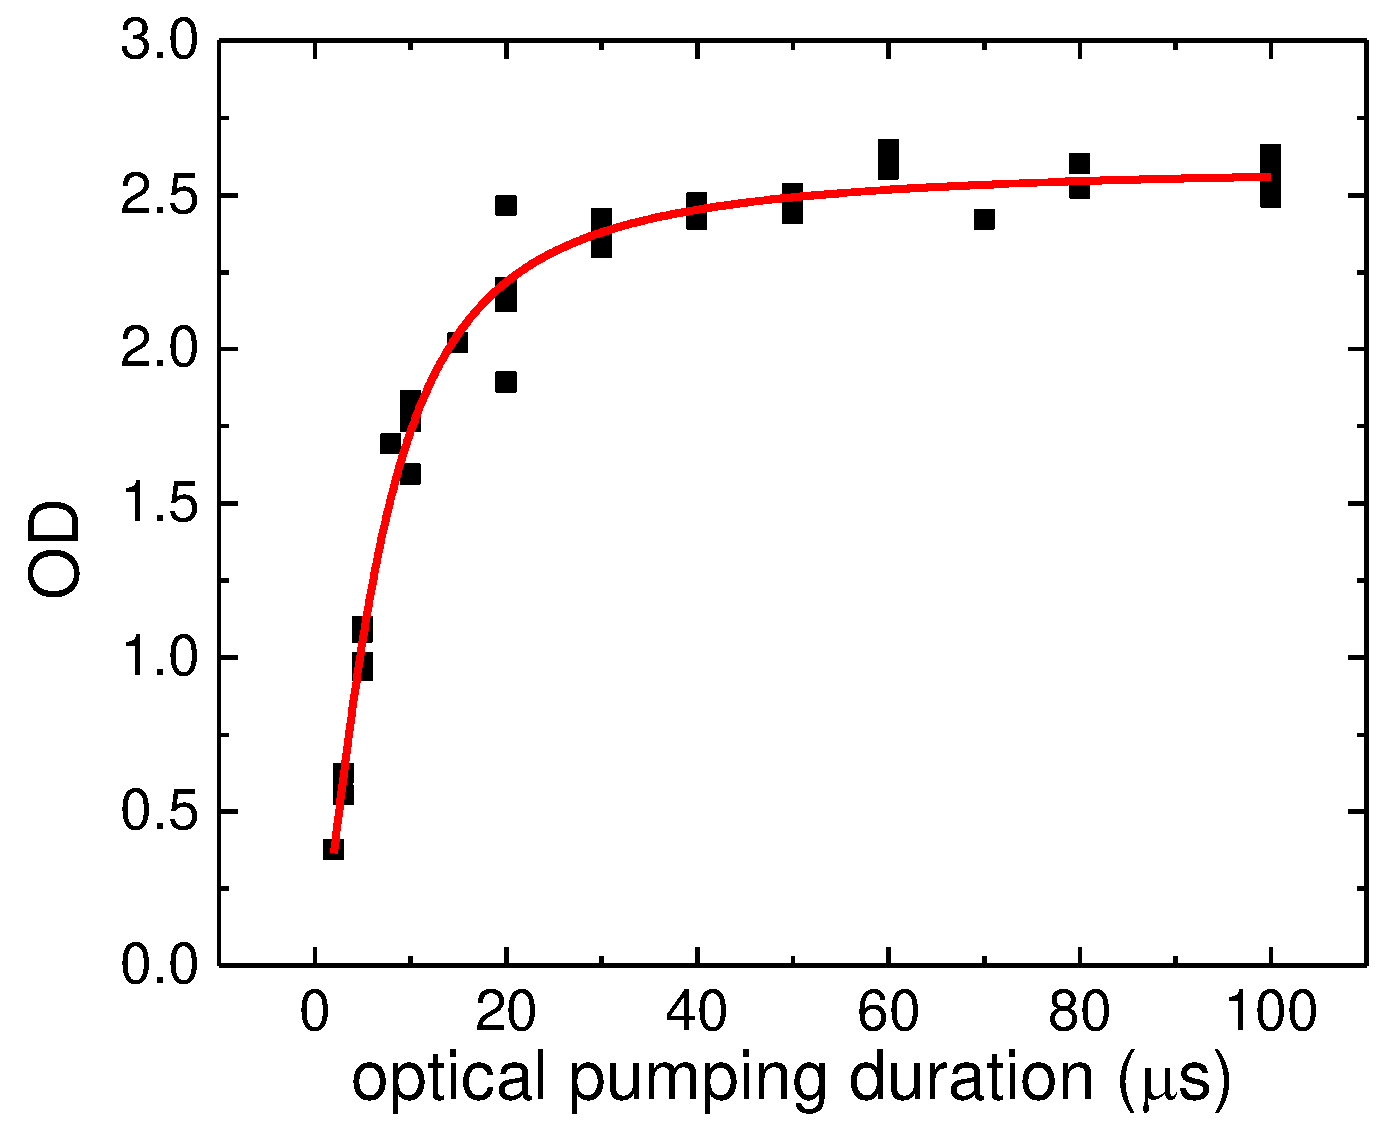
\includegraphics[width = 0.8\linewidth]{figures/partial_pumping.pdf}
\end{center}
\caption[Partial pumping portion as function of pump duration]{Partial pumping portion as a function of pump duration. Here shows the partial pumping for Na with 200 MHz blue detuning of the pumping light.}
\label{partial pumping}
\end{figure}

\subsection{Atomic number calibration}

% overall and method(done 2021-9-20 11:47:23)
In the previous subsection \ref{subsec:high_mag_absop_image}, in order to perform absorption imaging on samples with higher optical density (OD), we use the partial pumping method to reduce its OD. However, in order to ensure the signal-to-noise ratio of the imaging, we usually do not use the probe light whose intensity is much smaller than the saturation intensity. Therefore, considering that the droplet experiment requires atomic number measurement, we need to do a more careful atomic number calibration for our high field absorption imaging. The principle of calibration is mainly derived from the calibration of several parameters in absorption imaging. For now weak probe light intensity, the expression of absorption imaging is
\begin{equation}
\frac{dI(x,y)}{dz}=-n(x,y,z)\sigma_{eff}(\delta,I,others)I(x,y)
\end{equation}
In above formula, $\sigma_{eff}$ represents the effective cross-section of atoms, which is related to probe detuning, intensity and other parameters such as polarization. By separating intensity and detuning, we have
\begin{equation}
\sigma_{eff}(\delta,I,others)=\frac{\sigma^*(others)}{(1+(\frac{2\delta}{\Gamma})^2)+\frac{I}{I^*_{sat}(others)}}
\end{equation}
Probe light transmits along the $z$ direction and has a distribution in $x$-$y$ plane. $n(x,y,z)$ is density distribution of a bulk sample. When we do absorption image, we actually probe the column density
\begin{equation}
\label{sat_absorp_formula}
\int n(x,y,z)dz=\frac{OD(x,y)}{\sigma^*(others)}=\frac{1}{\sigma^*(others)}[ln(\frac{I_{in}}{I_{out}})+\frac{I_{in}-I_{out}}{I^*_{sat}(others)}]
\end{equation}
Thus, in the following calibration, we mainly calibrate two parameters: $I^*_{sat}(others)$ and $\sigma^*(others)$.

% calibrate saturation intensity: beta (done 2021-9-20 23:29:58)
First, we follow \cite{reinaudi2007strong} to calibrate $I^*_{sat}(others)$, which we called it $\beta$-calibration. We define
\begin{equation}
I^*_{sat}(others)=\beta I^0_{sat}
\end{equation}
where $I^0_{sat}=\frac{\hbar \omega A_{21}}{2 \sigma_0}$ is the ideal saturation intensity. To calibrate the beta, we use different camera light intensities to probe the same sample and then directly plot the od without correlation, i.e. $ln(\frac{I_{in}}{I_{out}})$. As shown in Fig. \ref{Image_beta_calibration}, the y-axis represents the counting rate of probe light which is proportional to light intensity $I_{in}$; x-axis is the od without correction we mentioned before. Via formula \ref{sat_absorp_formula} We can fit this curve and then get $CR_{sat}^{eff}$. We use counting rate instead of light intensity, mainly because CR can be read directly on the camera. Using the effective saturated CR to obtain the corrected od is more directly than using $\beta$. In other words, for the correction of imaging, we don't actually care about the value of $\beta$, and it is actually enough to have saturated CR. Finally, in Table. \ref{tab:image_cali}, we offer the effective saturated CR  of Na and Rb in the two different image systems we used. At the same time, we point out here that the $\beta$ value depends on various parameters, including light polarization, camera parameters, projection parameters of the imaging system, etc. Therefore, the number calibration of each system should be done separately. Through this engineering method, all unexpected parameters are absorbed into a single variable.

% Image_beta_calibration (done 2021-9-20 14:11:12)
\begin{figure}[htb]
\begin{center}
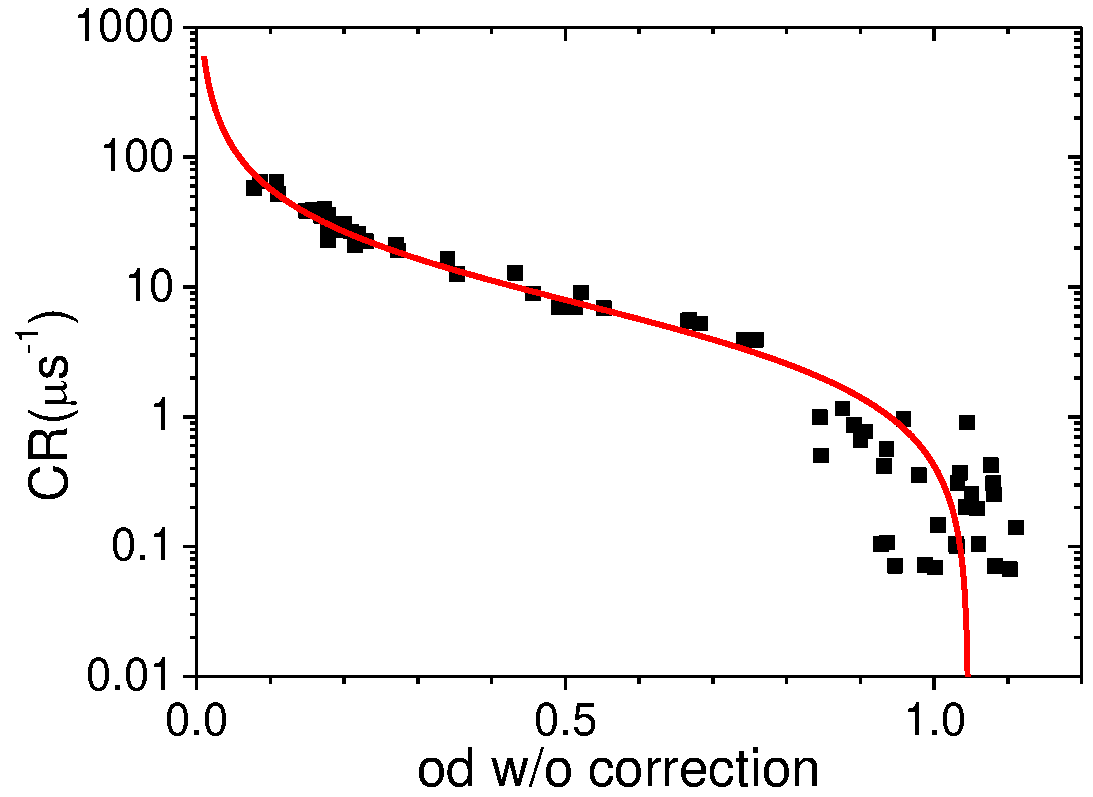
\includegraphics[width = 0.8\linewidth]{figures/Image_beta_calibration.pdf}
\end{center}
\caption[$\beta$-calibration of Rb 15x absorption image]{$\beta$-calibration of Rb 15x absorption image. CR is counting rate, i.e. average counting over probe duration. od w/o correction is $ln(I_{in}/I_{out})$ without correcting the saturation effect.}
\label{Image_beta_calibration}
\end{figure}

% calibrate alpha (done 2021-9-20 23:38:36)
The above calibration for saturated light intensity avoids the OD change of the sample from different probe intensities. However, considering the expression \ref{sat_absorp_formula}, in order to obtain the column density distribution of the sample, we also need an effective scattering cross-section $\sigma_{eff}$. In order to obtain this parameter, we need to compare the OD obtained by absorption image to the column density of the actual atom density distribution. The point to be emphasized here is that we do not use the parameters in the $\beta$-calibration to correct the cross-section because of light imperfection, such as polarization, etc. The two are not entirely consistent. On the other hand, we use the partial pumping method. Therefore, we hope that this effective cross-section parameter can absorb the imperfection of pumping, such as leakage to the other states, which does not result in 100\% pumping. We put this part of the calibration into the alpha. This part will not affect the saturation intensity of the probe but will affect the number of atoms counted at the end.

% methods of alpha calibration (done 2021-9-21 08:59:23)
For $\alpha$-calibration, we define
\begin{equation}
\sigma^*(others)=\frac{1}{\alpha} \sigma^0_{sat}
\end{equation}
Two methods can be used: one is from \cite{hung2011situ}, which directly compare the density distribution of BEC in-trap with, and directly compare the density distribution of the atom calculated by trap freq with the OD distribution obtained from the photo to obtain the corresponding $\alpha$-coefficient. The other is the number of atoms obtained through the BEC-thermal phase transition and the thermal part's temperature measurement. The corresponding alpha coefficient is obtained by comparing the total OD measured by the photo. The former method is more feasible for a sample with a larger in-trap size because the in-trap sample is typical $\mu$m level, which is difficult to avoid the impact due to the imaging resolution. The latter method can avoid this problem because the measurement of the total atomic number can be obtained from longer ToF. Therefore, in our experiment, we finally adopted the latter one.

% 待补充
% method BEC-thermal transition
% BEC-thermal的phase transition和原子数以及温度的关系是

% summary (done 2021-9-23 11:58:33)
In general, through the above two steps, we can accurately obtain the density distribution of the atom. Adding the high-field imaging method introduced in the Subsec. \ref{subsec:high_mag_absop_image}, we finally offer a complete imaging plan for the droplet experiment. This solution is also suitable for in-situ imaging samples with relatively high OD, such as in-trap BEC, bright solitons, etc. Furthermore, achieving enough resolution by upgrading the imaging system is essential as another aspect of the requirement to retrieve density distribution.

% CR and alpha table (done 2021-9-23 11:58:46)
\begin{table}[]
\begin{tabular}{|l|l|l|l|l|l|l|l|l|}
\hline
   & \begin{tabular}[c]{@{}l@{}}Image\\ system\end{tabular} & \begin{tabular}[c]{@{}l@{}}Mag.\\ field\end{tabular} & \begin{tabular}[c]{@{}l@{}}Probe\\ polar.\end{tabular} & \begin{tabular}[c]{@{}l@{}}OP\\ det.\end{tabular} & $CR_{sat}^{eff}$ & \begin{tabular}[c]{@{}l@{}}$I_{sat}$\\ (mW/$cm^2$)\end{tabular} & $\beta$ & $\alpha$ \\ \hline
Rb & 3x                                                     & LF                                                       & Circular                                               & 0 MHz                                             & 87(4)       & 2.792                                                           & 1.67    & 1.59     \\ \hline
Rb & 15x                                                    & HF                                                       & Horizo.                                                & 0 MHz                                             & 5.7(3)      & 5.421                                                           & 3.25    & 3.75     \\ \hline
Rb & 15x                                                    & HF                                                       & Horizo.                                                & 215MHz                                            & 5.7(3)     & 5.421                                                           & 3.25    & 4.54     \\ \hline
Na & 3x                                                     & LF                                                       & Circular                                               & 0 MHz                                             & 288(5)    & 5.862                                                           & 0.95    &          \\ \hline
Na & 15x                                                    & HF                                                       & Horizo.                                                & 140 MHz                                           & 24(1)     &                                                                 &         & 3.76     \\ \hline
\end{tabular}
\caption[Summary of image calibration]{Summary of image calibration}
\label{tab:image_cali}
\end{table}


\section{CAMIMA: a multi-camera and image process platform}
\label{sec:camima}

% What is CAMIMA and why we need to develop it? (done 2021-8-27 18:27:20)
CAMIMA is a multi-camera control platform with image processing functions. Thanks to various camera adaptors provided by the Image Acquisition Toolbox in MATLAB, CAMIMA can support multiple types of camera, including USB cameras from PointGrey, PCO and Migtex, Web camera and other general type of cameras. The primary time sequence is tailored for the absorption image for the cold atom experiment. However, it is very convenient to switch to other sequences such as fluorescence imaging. After acquiring images from the camera, there are extendable and programmable image processing functions for post-processing images. Users can easily re-program the time sequence and processing sequence for various scenarios, e.g. denoising or de-fringe process, fluorescence image and so on.

% components description (done 2021-8-27 18:41:59)
The software is made of four parts: 
\begin{itemize}[noitemsep,topsep=0pt]
\item CAMIMA: Main control for converting data from different camera to a uniform image stream, which easier for following processing.
\item VUIMA: For showing and processing images from each image stream. VUIMA can be opened multiple.
\item CAMSET: Setting program for various cameras. Inside it, there is a general setting panel adaptation for specific type of camera.
\item FITSET: For general purpose fitting progress. fitting function can be edited as will.
\end{itemize}

\subsection{licensing, versions and updates}
% licensing (done 2021-8-27 18:42:40)
This programs is a free software: you can redistribute them and/or modify them under the terms of the GNU General Public License, version 3, as published by the Free Software Foundation. The full text of the license is available from \href{https://www.gnu.org/licenses/}{https://www.gnu.org/licenses/} and is included in the file COPYING included in the distribution.

% Version control (done 2021-8-27 18:42:47)
For adapting different version of MATLAB and its Appdesigner toolbox, CAMIMA can run under following versions:
\begin{itemize}[noitemsep,topsep=0pt]
\item MATLAB2016
\item MATLAB2020
\end{itemize}

% download and updates (done 2021-8-27 18:42:51)
Software downloads and updates are made available via github:
\begin{itemize}[noitemsep,topsep=0pt]
\item \href{https://github.com/guozc12/CAMIMA}{https://github.com/guozc12/CAMIMA}
\end{itemize}

\subsection{Using the software: a basic guide}
\subsubsection{Prerequisites}
% prerequisite (done 2021-8-27 18:43:49)
Before installing CAMIMA, one need to install MATLAB with a version later than 2016. The listed several add-ons are needed.
\begin{itemize}[noitemsep,topsep=0pt]
    \item MATLAB (later than Ver. 2016)
    \item Appdesigner™ in MATLAB
    \item Image Acquisition Toolbox™ in MATLAB
    \item uitree in MATLAB
\end{itemize}

\subsubsection{Start CAMIMA}
% add Camima_main, i.e. main interface (done: 2021年8月4日21:43:37)
\begin{figure}[htb]
\begin{center}
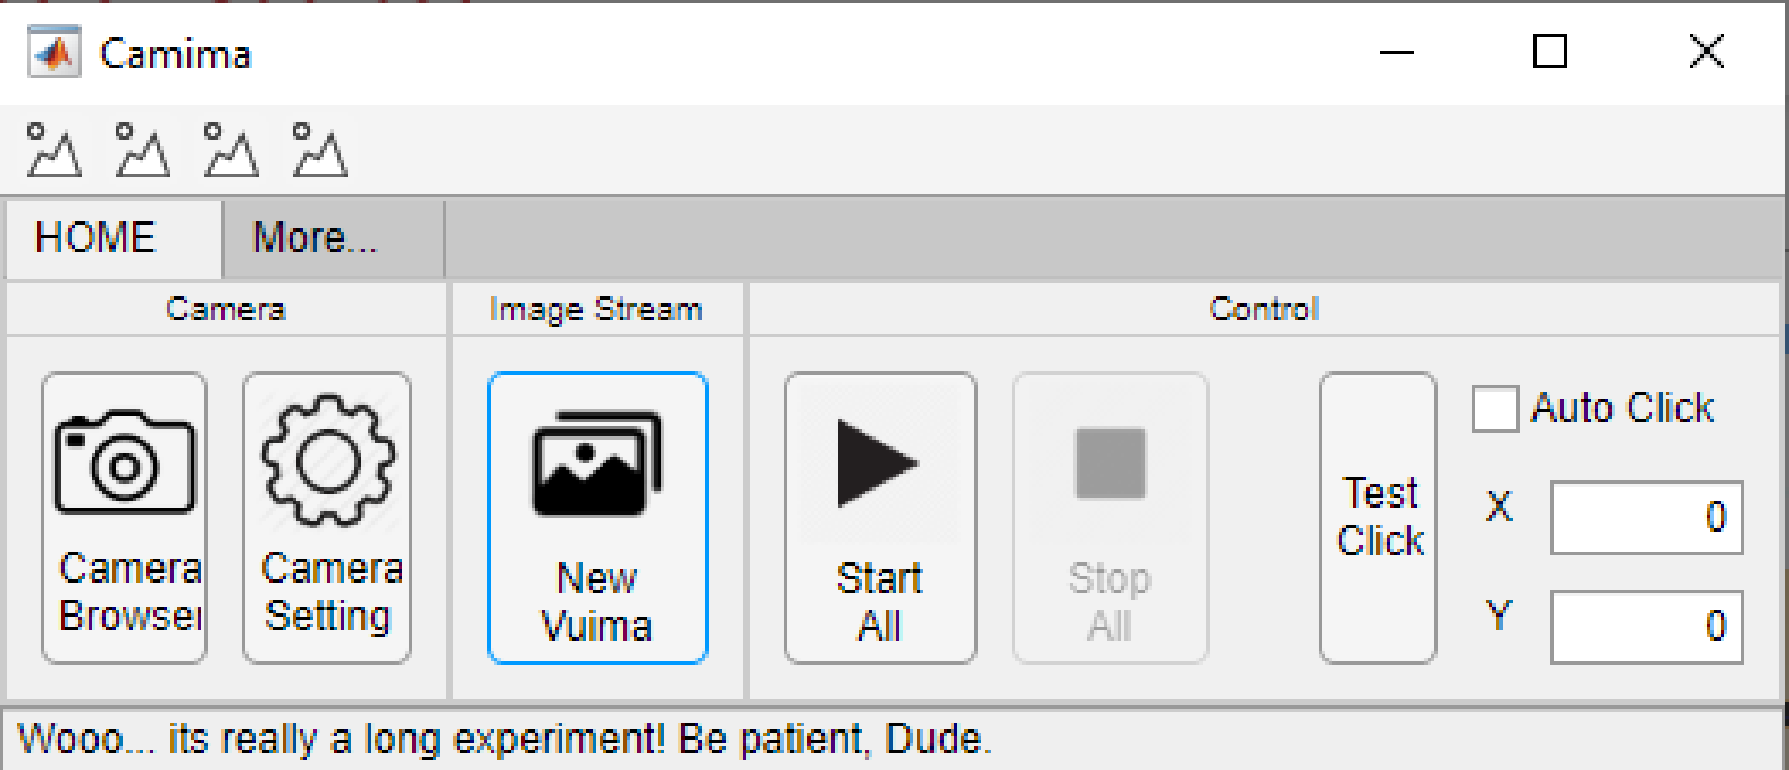
\includegraphics [width = 0.8 \linewidth]{Camima_main.pdf}
\end{center}
\caption[CAMIMA main panel]{CAMIMA Main panel.}
\label{Camima_main}
\end{figure}

% introducing the main panel (done: 2021年8月4日21:43:48)
Open the CAMIMA.mlapp in Appdesigner. Then click the Run button to run the main CAMIMA program. As shown in Fig. \ref{Camima_main}, a small panel shows you entrances for different functions:
\begin{itemize}[noitemsep,topsep=0pt]
    \item Camera Browser: Open a new panel for searching and initializing all installed cameras. (As shown in Fig. \ref{Camima_CamTree})
    \item Camera Setting: Open a new panel (CAMSET) to control each camera directly. (Fig. \ref{Camima_Camset})
    \item New VUIMA: Open an image processing panel (VUIMA) for viewing images and automatic image processing. (Fig. \ref{Camima_Vuima})
    \item Start All: For quick starting everything, including start acquisition for every camera
    \item Stop All: For quick stopping everything.
    \item Test Click: for setting a button, click after each shot with the written position on the right side.
\end{itemize}

\subsubsection{Setting cameras by CAMSET}
% camera adaptors for different venders

% add Camima_CamTree, i.e. Camera browser (done 2021-8-29 11:57:06)
\begin{figure}[htb]
\begin{center}
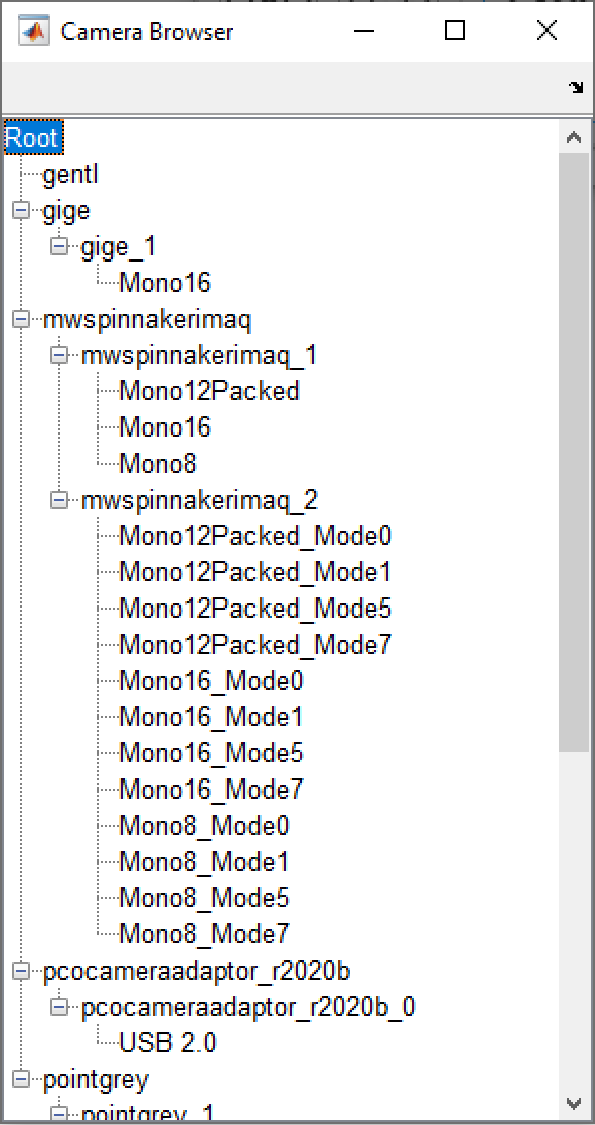
\includegraphics [width = 0.4 \linewidth]{figures/Camima_CamTree.pdf}
\end{center}
\caption[CamTree: show all available cameras for acquiring images]{CamTree shows all available cameras for acquiring images. When click the ``Camera Browser'' button in CAMIMA main panel, this tree window pops up and show you a full list of all available cameras.}
\label{Camima_CamTree}
\end{figure}

% Control the camera (2021-9-14 16:58:49)
As shown in Fig. \ref{Camima_Camset}, after catching each camera, we can control the camera manually, such as previewing, get a snap by the manual trigger and setting various parameters controlling the camera. For cameras from different vendors, the general settings are different. Thus, we generate a list in a new window, as shown in the right panel of Fig. \ref{Camima_Camset}. Users can change the private properties of the camera, such as exposure time, binning and other higher-level parameters. The ROI (Region-of-interest) can only be set when the camera is stopped as shown in the right-middle of CAMSET panel. Parameters for automatic triggering can be set in the right-bottom panel of the CAMSET window. By the way, as we mentioned before, our program can support various types of cameras which is listed as follows:

% Types of camera supported (2021-9-14 17:33:16)
\begin{itemize}[noitemsep,topsep=0pt]
    \item PointGrey USB camera
    \item BlackFly USB camera
    \item PCO USB camera
    \item camera with GIGE (web cam)
    \item other general types of camera
\end{itemize}

% add Camima_Camset, i.e. Camera setting (done 2021-8-29 11:50:03)
\begin{figure}[htb]
\begin{center}
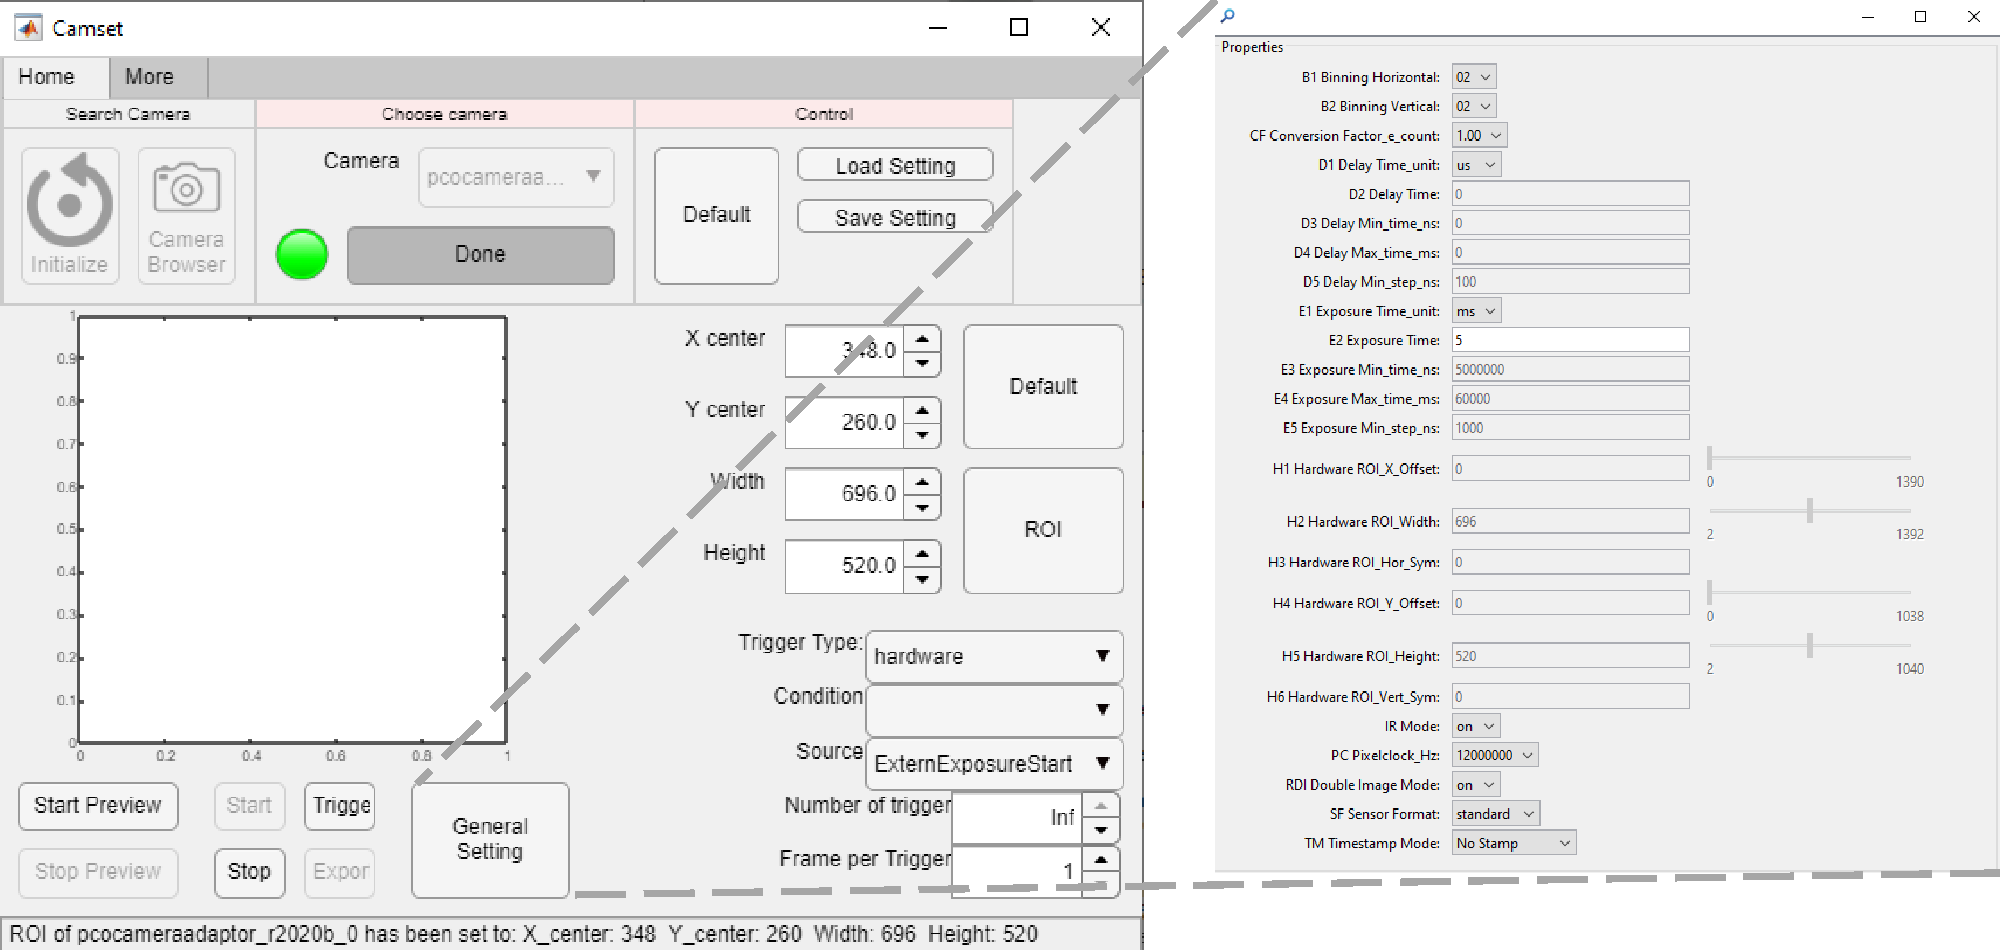
\includegraphics [width = \linewidth]{Camima_Camset.pdf}
\end{center}
\caption[CAMSET: a module of CAMIMA used to control and set cameras]{CAMSET is a module of CAMIMA used to control and set cameras. By switching the toggle, one can control multiple cameras. Besides the general setting, such as ROI and acquisition sequence, it also offers a specific entrance for each camera.}
\label{Camima_Camset}
\end{figure}

\subsubsection{Image acquisition}

% add Camima_Vuima, i.e. Viewing the image (done 2021-8-29 11:46:52)
\begin{figure}[htb]
\begin{center}
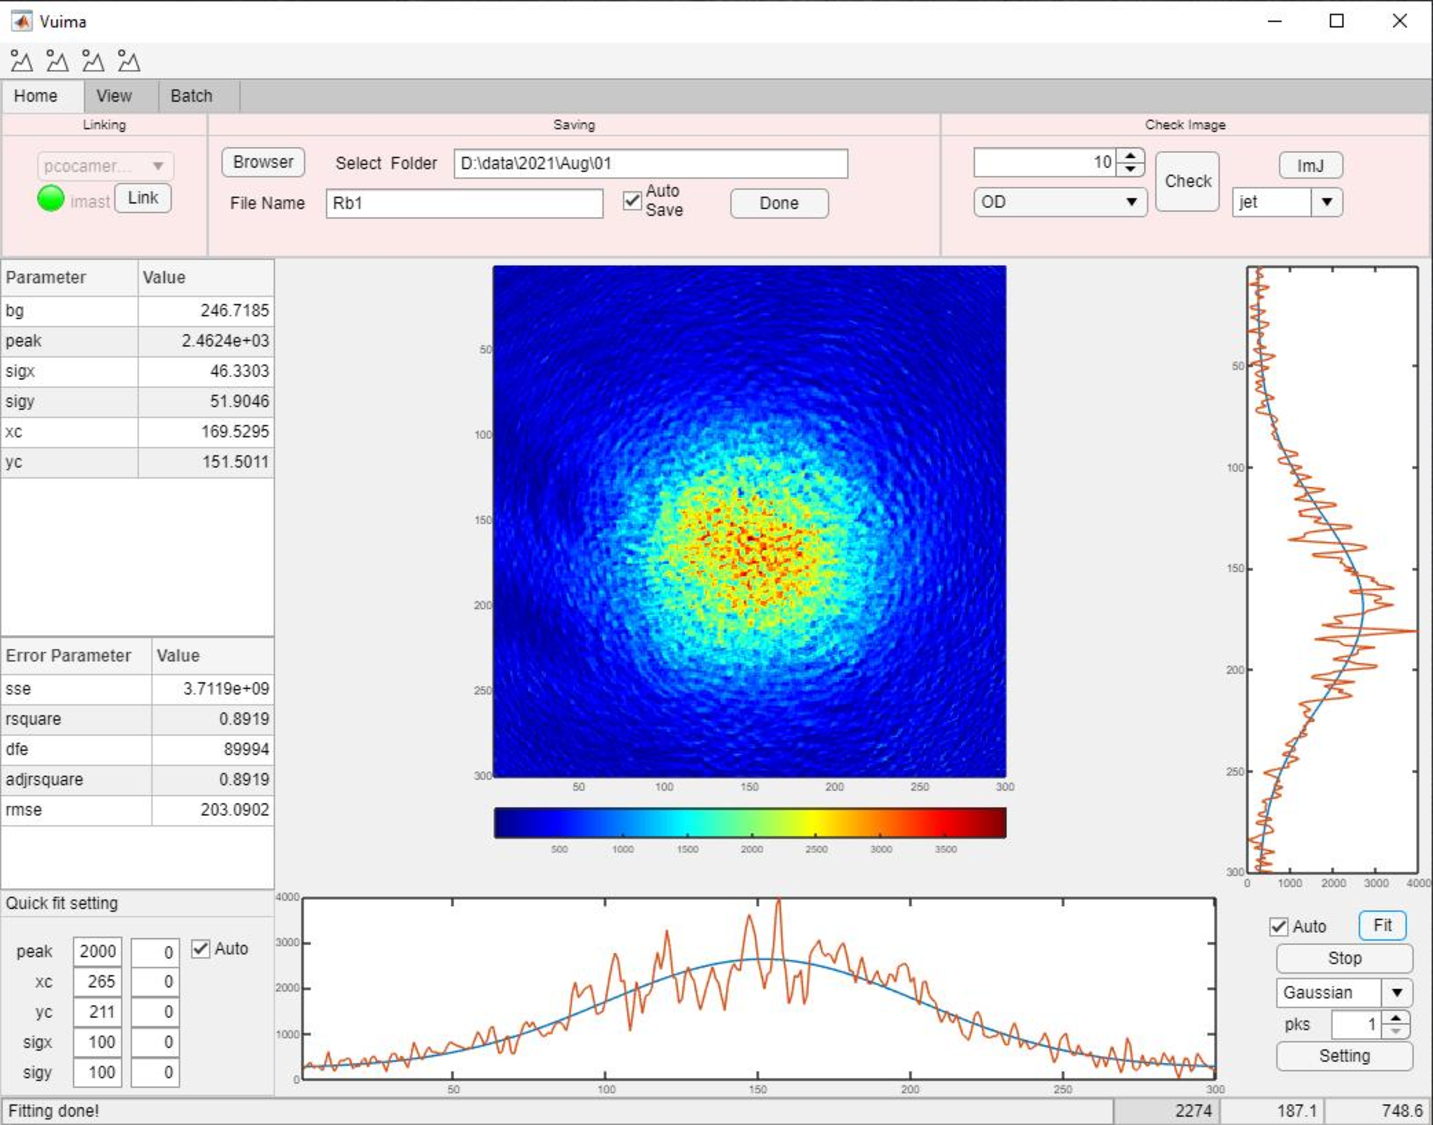
\includegraphics [width = \linewidth]{Camima_Vuima.pdf}
\end{center}
\caption[VUIMA: a module of CAMIMA used to preview image]{VUIMA is a module of CAMIMA used to preview image. The VUIMA window can be opened multiple for each image stream. Besides previewing the image, it can show the fitting results comparing to the raw data. It offers entrance for setting arbitrary fitting function.}
\label{Camima_Vuima}
\end{figure}

% time sequence of image acquisition (done 2021-9-16 20:33:38)
After configuring the camera, the platform is ready for automatic image acquisition. By setting the trigger, we can integrate the camera as part of the control system. For absorption imaging, we take three pictures for each imaging, which is achieved by setting three triggers to the camera. The picture will be temporarily cached in memory. Trigger the event by setting the number of triggers. For example, after receiving three triggers, start processing the absorption imaging picture and calculate the OD picture. For specific details of absorption imaging, please refer to that section. When we have multiple cameras that need acquisition data, each camera can complete the data collection independently.

% converting camera data to image stream (done 2021-9-16 20:38:54)
Some cameras, such as PCO, have a double image. Then, we need to divide the data collected by the camera. In order to ensure the versatility of subsequent image processing and avoid the need for different codes for different cameras, we use an adaptor to convert the raw data from cameras to independent image streams. The settings of the camera and the acquisition of the camera are in the \textit{camera stream}. Then it generates image streams. For example, a single imaging camera only provides one image stream, while a PCO double-image camera can provide two image streams. Select a specific image stream to do subsequent processing. In this way, we can say that a specific image stream is displayed in a window, i.e. VUIMA.

% show and pre-process of images on VUIMA (done 2021-9-16 21:02:31)
One VUIMA is connected to one image stream. Users can select the existing image stream in the link in the upper left corner of the VUIMA panel. As the collected images are generated, VUIMA is responsible for pre-processing the images. The statistical data will be given in the lower right corner, including the number of photons in pure light photos, by setting the exposure time, calculating the light intensity, and giving a preliminary count. For the three images collected, the data needs to be cleaned first. VUIMA first removes abnormal points and take average around them. Then it processes the OD images. Because the Log function is used, in order to avoid too many abnormal values, we adopt the cut-Log method to treat points with OD smaller than -0.2 as 0. This works for most pictures and can detect abnormal cases when sometimes the trigger is broken. For some pictures with a low signal-to-noise ratio, this limit can be modified to a lower value to ensure the authenticity of the data. Subsequently, the processed OD picture will be displayed in the middlebox, and fitting will be carried out simultaneously. The fitting result displays on the right and bottom of Vuima, in the form of slices along with the raw data points. The specific fitting will be introduced in the next section.

\subsubsection{post processing of image}

% add Camima_Fitset, i.e. Setting the fitting (done 2021-8-29 11:54:52)
\begin{figure}[htbp]
\begin{center}
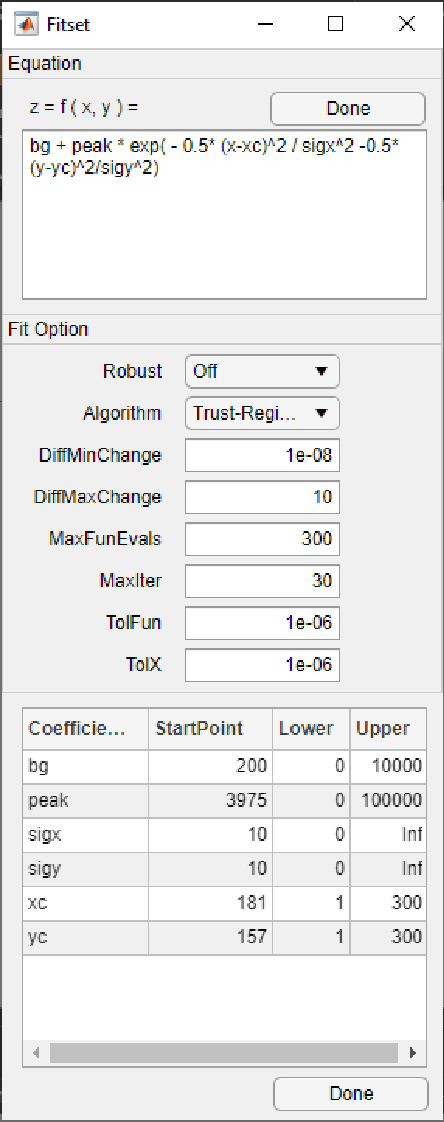
\includegraphics [width = 0.4\linewidth]{Camima_Fitset.pdf}
\end{center}
\caption[FITSET: a module of CAMIMA used to set arbitrary fitting function]{FITSET is a module of CAMIMA used to set arbitrary fitting function. Besides the default fitting functions written under the toggle button, this module offers function for easily generate arbitrary fitting function.}
\label{Camima_Fitset}
\end{figure}

% fitting of image (done 2021-9-16 21:18:21)
We first perform preliminary fitting on the collected pictures. The fitting function can be selected in the panel in the lower right corner of VUIMA. Thermal sample adopts 2D-Gaussian, BEC adopts parabola and so on. Multiple peaks can be selected. For mixed samples, one can choose a mixed model. At the same time, a user-defined module can be opened in the FITSET window. The general fitting takes typical 3-10 seconds, which can ensure that the analysis result can be obtained immediately and the decision can be made within a shot. Of course, Users can try to increase this speed. For the peak model, whether single-peak or multi-peak, one can manually select the initial value or automatically select the initial value. You can see the initial value selection in the lower-left corner of the Vuima panel. As the peak increases, more blanks can be added. The fitting result will also be stored in a CSV file for real-time import to the origin to give further analysis, such as temperature, number, density, and other parameters. At the same time, it is very convenient to compare multiple shots, draw pictures, etc.

% statistic data from image (done 2021-9-16 21:26:40)
The fitting data is first displayed in the table on the left. Users can get fitting errors by sliding the form to the left. In addition, indicators such as r-square value are given in the middle on the left. Adj-square is used to indicate which model is better to use when the model is not clear. In order to facilitate the data analysis after the experiment, Vuima has developed a batch processing module for batch processing of a large number of pictures. Because of the convenience of programming, this function has a high degree of freedom, and users can freely add the codes they want to process in the module.


\subsection{Vision and outlooks}

% Vision (done 2021-9-16 21:31:37)
From the perspective of experimental physics, there are two primary purposes for using or developing new technologies: The first is to detect physical quantities that were previously undetectable through technological advancement. The second is to improve the efficiency of experiments and work through technological advancement. The former makes the frontiers of experimental physics one step forward, while the latter can make experiments one step further away from industrialization. Cold atom physics has been developed for more than two decades. Nowadays, with the rise of quantum computing, it is time to consider further substituting industrialization methods into experimental research to pave the way for research-industry transformation.

% Purpose of developing the program (done 2021-9-16 21:35:49)
Strictly speaking, CAMIMA is only the second half of the entire cold atom experiment timing system, which is the data acquisition part. A complete experiment sequence system should be able to record all the data of each experiment: including sequence setting parameters, checking and testing parameters. Generally, we will focus the laboratory data on only what we want to control, such as a specific frequency or power, and what we want to see, such as absorption imaging pictures. However, all measured quantities are part of the experiment. A complete record has two advantages: First, a complete record includes complete monitoring, which can avoid out-of-control conditions. Second, a complete record can make the data of each shot more valuable. For example, the data collected on different days is comparable. Through systematic data analysis, there will be unpredictable discoveries. Furthermore, these are inseparable from introducing new, efficient data acquisition technology and data analysis and processing technology. In general, martial arts in the world can only be broken quickly. The pursuit of efficiency is the eternal theme of science and research.

\section{Fast magnetic field control}
\label{sec:fastcoil}

% why we need fast-magnetic control (done 2021-9-16 22:33:50)
As we mentioned in the section about Feshbach resonance, by tuning the magnetic field, we can easily control the scattering properties of atoms, i.e. the interaction strength. In the previous set-up, we use a large Helmholtz coil with 70 turns. The coil's inductance is three mH, which is huge, introducing a significant time constant. So, even using a driver with 100V(check), we will have a rising slope of about 1 ms, which is not fast enough for our requirement to control the interaction. Our request depends on the time scale of the research object. For example, a typical BEC with a scattering length of 100 $a_0$ order will have a time scale of less than 1 ms. Thus, we need a new magnetic field control system with the time scale of $\mu$s level to control the interaction fast. Then we can make sure the sample's size of other parameters changing much slower than the interaction changes.

% fast coil design (done 2021-9-23 11:59:31)
\begin{figure}[htb]
\begin{center}
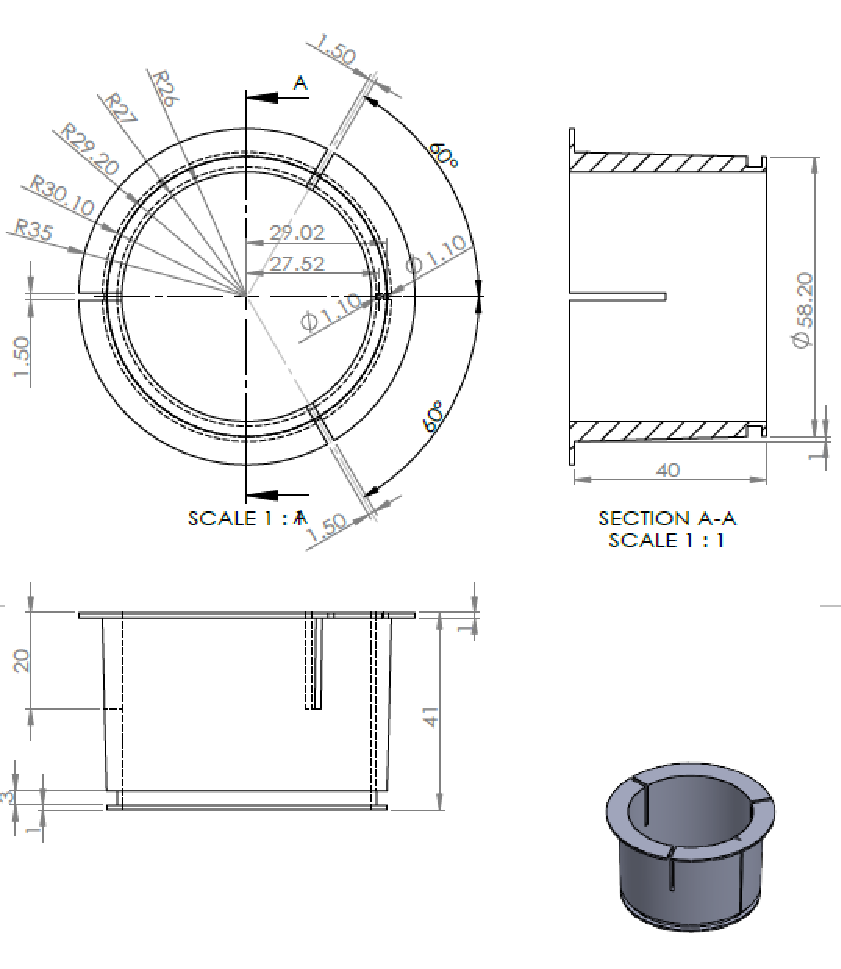
\includegraphics [width = 0.6\linewidth]{Apparatus_coil_holder.pdf}
\end{center}
\caption[Fast coil holder]{Fast coil holder for adapted to existing main coil system.}
\label{Apparatus_coil_holder}
\end{figure}

% What is fast coil and how to build one. (done 2021-9-16 22:41:19)
So, with the above request, we need to build another coil that can generate a small but fast magnetic field. The limitation is the coil's inductance, so we reduce its turns to as few as possible. However, with fewer tunes, the magnetic field can generate a less magnetic field. So we need to make a trade-off here. Finally, we choose a diameter 60 mm coil pair with six turns for each one. Also, to generate a larger magnetic field, we put it as close as possible to the cell. The set-up with the main Feshbach coil is shown in Fig. \ref{Apparatus_coils}. To adapt our previous large coil, we designed a holder made of polyvinyl as shown in \ref{Apparatus_coil_holder}. Moreover, the holder winding with the fast coil is inserted into the 2-inch optical path to avoid blocking the MOT beam.

% current driver and its test data (done 2021-9-17 10:21:11)
To drive this fast coil, we need a current driver that fast turns on/off and makes a precision control of the current with tiny leaking current. So, with Lintao's help, we design a fast coil driver with two groups of JFET. Each group is several JFETs set in cascade. This design uses the intrinsic fast-changing property of JFET compared to MOSFET, which typically possesses large junction capacitance. Also, cascade sets of JFETs can reduce the leak current from the base since after several levels the current in the base can be reduced to $\mu$A level or even better. The driver schematic and simulation by Tina-TI can be found in the appendix. \ref{chap:M&E}.

% fast coil couple with main coil and environment (done 2021-9-23 12:02:43)
\begin{figure}[htbp]
\begin{center}
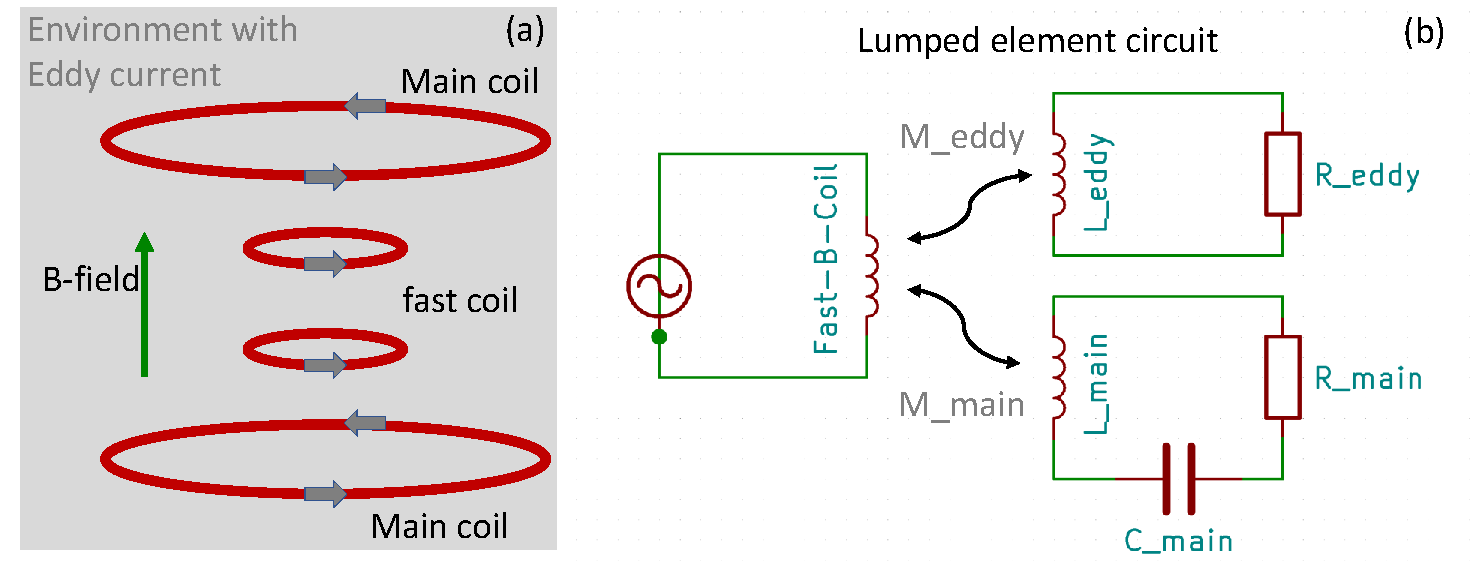
\includegraphics [width = \linewidth]{Apparatus_coils.pdf}
\end{center}
\caption[Fast coil, main coil and environment]{(a) set-up with main coil for generating hundred-Gauss level magnetic field and fast coil can change magnetic field in $\mu$s time scale. There is also the coupling between these coils and environment, such as metal optical board around the coil or cables for connecting antennas. (b) Lump circuit for simulating the system with two coils and the environment.}
\label{Apparatus_coils}
\end{figure}

% design of fast coil (done 2021-9-21 21:55:54)
Two parts of the fast coil are put as close as possible to avoid introducing more curvature since the cell is too large for the Helmholtz condition. Finally, the fast coils are separated 70 mm with a diameter of 60 mm. Each coil has an inductance of less than 5 $\mu$H. This enables us to generate a magnetic with a slew rate larger than 500 G/ms. In other words, we can change the magnetic field with several $\mu$s when working around the Feshbach resonance. As shown in Table. \ref{tab:coils}, by injecting 1 A, we can get 0.67 G (set in Helmholtz type). Our current controller can bear a surge current of less than 10 A as we use two TIP31. So, finally, we can get a maximum magnetic field of 6.7 G which is definitely enough as a fast trim in daily experiments.


% add table here about fast coil and main coil (done 2021-9-21 21:56:05)
\begin{table}[htbp]
\centering
\begin{tabular}{|l|l|l|}
\hline
                        & Main coil      & Fast coil             \\ \hline
Coil sepa. to atom (mm) & 25 – 85        & 35                    \\ \hline
Coil radius (mm)        & 52 – 90        & 30                    \\ \hline
Coil inductance         & $\sim$3 mH     & $\sim$5 $\mu$H        \\ \hline
Magnetic field per A    & $\sim$8.2 G    & $\sim$0.67 G          \\ \hline
Ramp speed              & $\sim$0.6 G/ms & \textgreater{}500 G/ms\\ \hline
Number of turns         & 70             & 6                     \\ \hline
\end{tabular}
\caption[Parameter table of main coil and fast coil]{Parameter table of main coil and fast coil}
\label{tab:coils}
\end{table}

% coupling of fast coil and main coil (done 2021-10-28 17:19:01)
As explained in \cite{cumby2012exploring}, we need to consider the coupling of the fast coil, the main coil and the environment. Since, these coupling will cause oscillation and jiggle when quenching the current in the fast coil. As modeled by the lump elements, as shown in Fig. \ref{Apparatus_coils}. The Fast coil are simulated as a inductance driven by a current source. fast coil has mutual inductance with main coil and the environment. The main coil is viewed a RLC circuit and the environment only as a RL circuit. With this lump circuit simulation, we can qualitatively figure out however these three things coupled to each other. However, more detailed parameter can only be achieved by measure the response of the system. By adding a quenching signal, we can get the response of the whole system. Then, we can do feed-forward to compensate the overshooting or jiggles since the speed of fast coil is about 1000 times faster than the Main coil and the environment.

% Why we need dynamic compensation
There are two reasons for us to do the dynamic compensations, first is the coupling of the fast coil and main coil, and the environment will cause a jigger when we quench the current of the fast coil. To avoid this jigger, we feed-forward set the current to compensate for this overshooting. The second is for the droplet experiment: because the magnetic field generated by the main Feshbach coil has a gradient, when we do ToF, the magnetic field at atom position changes with time. So, to keep the magnetic field on atoms unchanged with ToF, we need this dynamic compensation. For the first case, the compensation needs very fast, so we use the fast coil. For the second one, it is a relatively slow-changing process. So we only use the shim coil to do the compensation. 

\section{Other Technical Issues}
\subsection{Magnetic field gradient compensation}
\label{subsec:gradientcompen}

%Why we need to compensate the B-field gradient (done 2021-9-24 17:34:04)
As mentioned before, we use a pair of Feshbach coils to generate a large bias magnetic field to control the Feshbach resonance. However,  the imperfection of the coil, such as asymmetry of coils and imperfection of distance between up-down Helmholtz coils, renders a gradient and curvature of the magnetic field. This effect can be easily detected by the free-falling of atoms in the high magnetic field. If one finds that the atom's acceleration deviates from gravity acceleration, there must be a gradient. Another evidence is the MW (RF) spectroscopy for an elongated sample that could detect the horizontal gradient. When we free-falling Rb or Na under a high magnetic field, if the acceleration becomes different from gravity, we can use it as an indicator of magnetic field gradient.

% What is our gradient looks like? (done 2021-9-17 22:37:43)
Before talking about cancelling this gradient, we first measure it. The method is simple, following the MW transition calibration method, we apply the MW pulse coupling the $\ket{1,-1}$ and $\ket{2,0}$ state. To get the spatial distribution of the magnetic field, we first let the atom free-fall, then apply the MW pulse at different ToF. Even though the gradient affects the atom's position by adding an extra acceleration, considering the small effect related to gravity, this can be neglected. Not only exists the gradient but also the the curvature of the magnetic field because the spatial changing B-field is definitely more than linear. By a simple quadratic curve fitting, we get the curvature of about $2.47 \times 10^3$ G/cm$^2$ and an average gradient of about xx G/cm. One thing that needs to be noticed here is that we measured only the magnetic field gradient in the vertical direction, which is our main contribution. As we can see in the horizontal direction, the acceleration is even much lower than that in the vertical direction, which infer that this gradient should come mainly from the wrong distance of the Helmholtz coil.

% gradient compensation method
\begin{figure}[htb]
\begin{center}
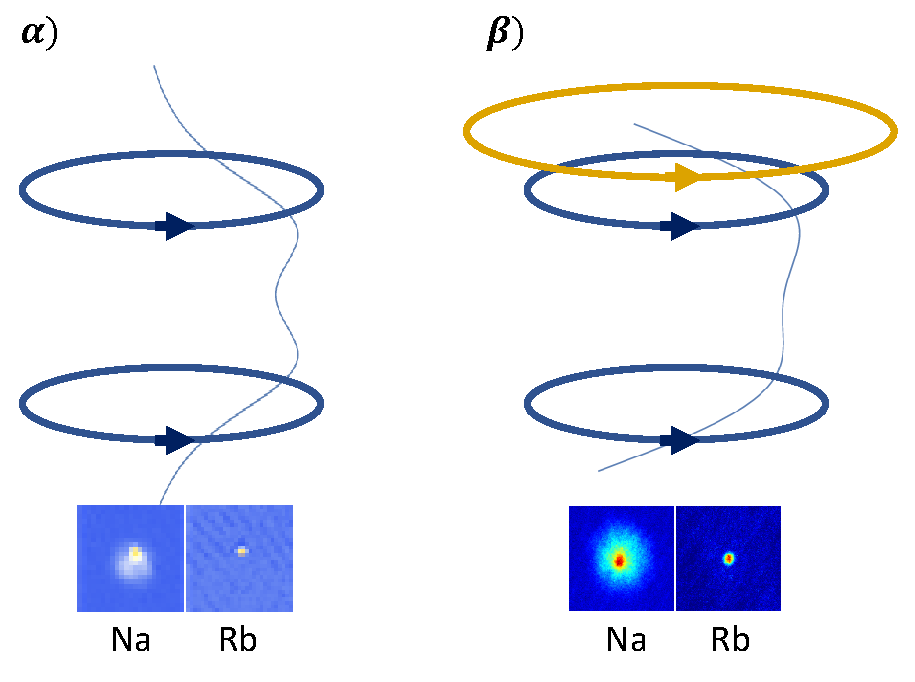
\includegraphics [width = 0.7 \linewidth]{Apparatus_gradient-compen.pdf}
\end{center}
\caption[Method of compensating the magnetic field gradient]{$\alpha$) B-field curvature and gradient affects free falling of atoms. $\beta$) Using only UP shim coil to compensate gradient.}
\label{Apparatus_gradient-compen}
\end{figure}

% How to compensate the gradient and curvature (done 2021-9-17 23:42:44)
It is hard to totally compensate the curvature because it will need to entirely recover the Helmholtz condition, which requires a much larger magnetic field to be added to the existing system. So, to solve the problem we meet, we degenerate to compensate the average gradient to zero inside the interesting ToF we care. So, we can add another magnetic gradient in the vertical direction and adjust its current to find the best compensation point. We use one of the up-down shim coil (e.g. up coil) as a preliminary test. As shown in Fig. \ref{Apparatus_gradient-compen}, we can generate an inverse direction gradient opposite to the main coil. 

% add find compensation point method (done 2021-10-28 18:17:22)
\begin{figure}[htb]
\begin{center}
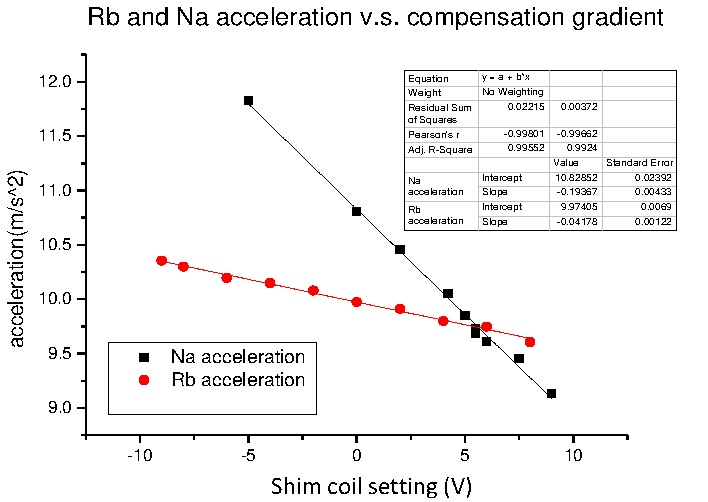
\includegraphics [width = 0.7  \linewidth]{Apparatus_compen_method.pdf}
\end{center}
\caption[Method of searching the compensation point]{By searching the cross point of Na and Rb sharing the same acceleration, we find the compensation point.}
\label{Apparatus_compen_method}
\end{figure}

% find the best compensation point (done 2021-9-17 23:54:51)
We change the current of the shim coil and test the acceleration of the atom to find the compensation point. As the dipole moment of Na and Rb is quite different, we can also find the intersect point of them, which represents zero average gradient compensation point, as shown in Fig. \ref{Apparatus_compen_method}. Finally, we tune the shim coil to the current at the intersection. We measure the magnetic field with the MW spectroscopy method and compare the result with the previous non-compensation one, as shown in Fig. \ref{Apparatus_mag_before_after}. It is evident that the mean gradient is reduced significantly; however, the curvature is still there. The compensated gradient on average (we take the 10 ms ToF as an average position) are about 0.11 G/cm, which should be enough to observe BEC mixture free-falling.

% before and after compensation measurement
\begin{figure}[htb]
\begin{center}
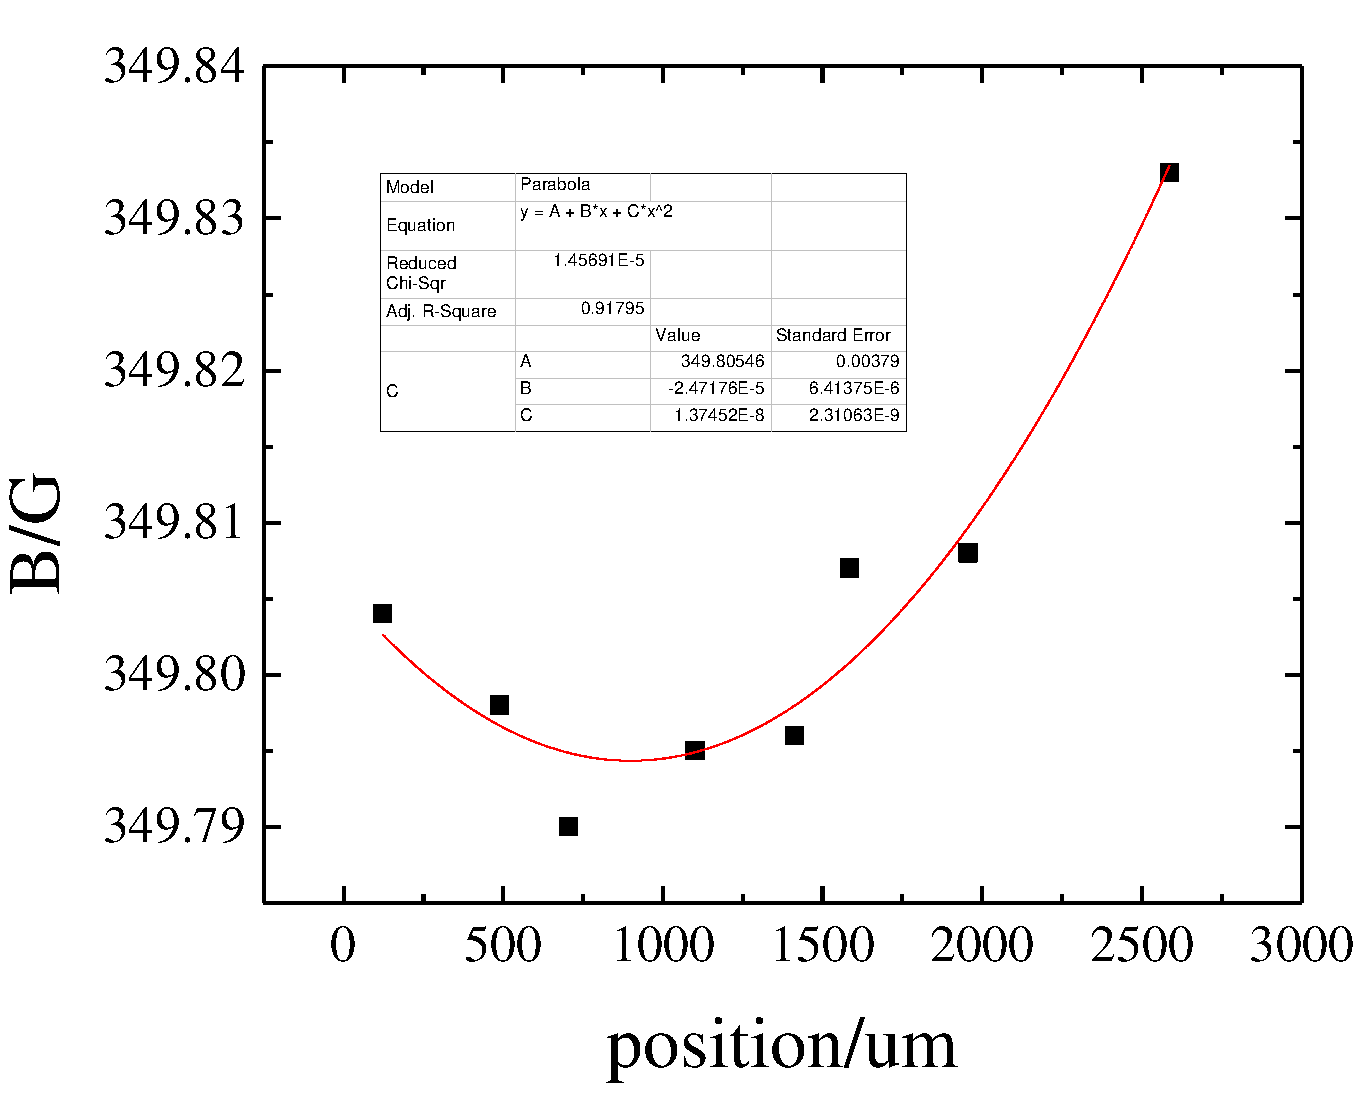
\includegraphics [width = 0.7 \linewidth]{Apparatus_mag_before_after.pdf}
\end{center}
\caption[Magnetic field spatial distribution at vertical direction after compensation]{Shows the magnetic field spatial distribution at vertical direction after compensation. It still remains gradient and curvature, however much smaller than the one before compensation. We fit it with a quadratic function to get the local gradient and curvature for compensation later.}
\label{Apparatus_mag_before_after}
\end{figure}

\subsection{Microwave full-wave loop antenna}
\label{subsec:FWLA}

% Why we need to build the 2.57GHz and 7.5GHz full-wave loop antenna (done 2021-9-22 00:15:26)
As described in SubSec. \ref{subsec:high_mag_absop_image}, the internal states of atoms can be controlled by the electromagnetic wave. Typically, to drive transition between two different hyperfine states, we need to use micro-wave(MW), which has a wavelength of about 0.3 m to 3 m, i.e. 300MHz to 300 GHz for frequency in the vacuum. The hyperfine splittings for Na and Rb atoms are 1.7 GHz and 6.8 GHz at zero magnetic fields. When the magnetic field increasing to 350 G (since we typically use the 347 G Feshbach resonance to control the inter-species interaction), the splitting between $\ket{F=1,m_F=1}$ and $\ket{F=2, m_F=2}$ states are 2.6 GHz and 7.5 GHz for Na and Rb separately. Thus, we need an antenna that can work well at this frequency. Here, ``work well'' commonly has two meanings: First, the antenna's standing wave ratio (SWR) is approaching 1, which means it can transmit most power to coil instead of reflecting it back to the power amplifier. Secondly, we need the atom to feel the largest amplitude of E-field because the transitions between different F-state is mainly connected by electron dipole, i.e. an electrical dipole transition. (here, need more carefully check) So, the antenna's position, including its distance to the atom and its direction angle, is critical to maximizing the utility of the antenna. We can define the efficiency for the above two processes as $\mu_{trans}$ and $\mu_{anta}$, and the total efficiency is just their multiplication.

% talk about near-field and far-field difference (done 2021-9-22 00:21:18)
A commercial antenna is typically designed to work well in the far-field region. The radiation power declines inversely proportional to the distance. Thus, to increase the power on the atom, we put the antenna to the atom as close as possible. However, this renders the radiation on the atom turns to be near-field instead of far-field. As depicted in Fig. \ref{antenna_EM}, the electric and magnetic field line of a dipole antenna is plotted as blue and red separately. At a considerable distance of the antenna, the electric field line is almost perpendicular to the \(\hat{r}\) direction. However, when getting closed, it shows more portions to the \(\hat{\theta}\) direction. This tells us that the near-field electromagnetic field of the antenna behaves quite different from its far-field one. Both electric and magnetic field lines are perpendicular to the Poynting vector in the far-field region, which shows its radiation properties. However, the near-field cannot be treated as radiation; instead, we typically treat it as a ``quasi-stati'' field. A quasi-static field means the distribution of EM field is the same as it in electrostatics, except an oscillation in magnitude with \(e^{i\omega t}\). In engineering, these study is essential to wireless-charging, proximity sensors and so on.

% near-field and far field EM field of antenna (done 2021-9-22 00:26:56)
\begin{figure}[htb]
\begin{center}
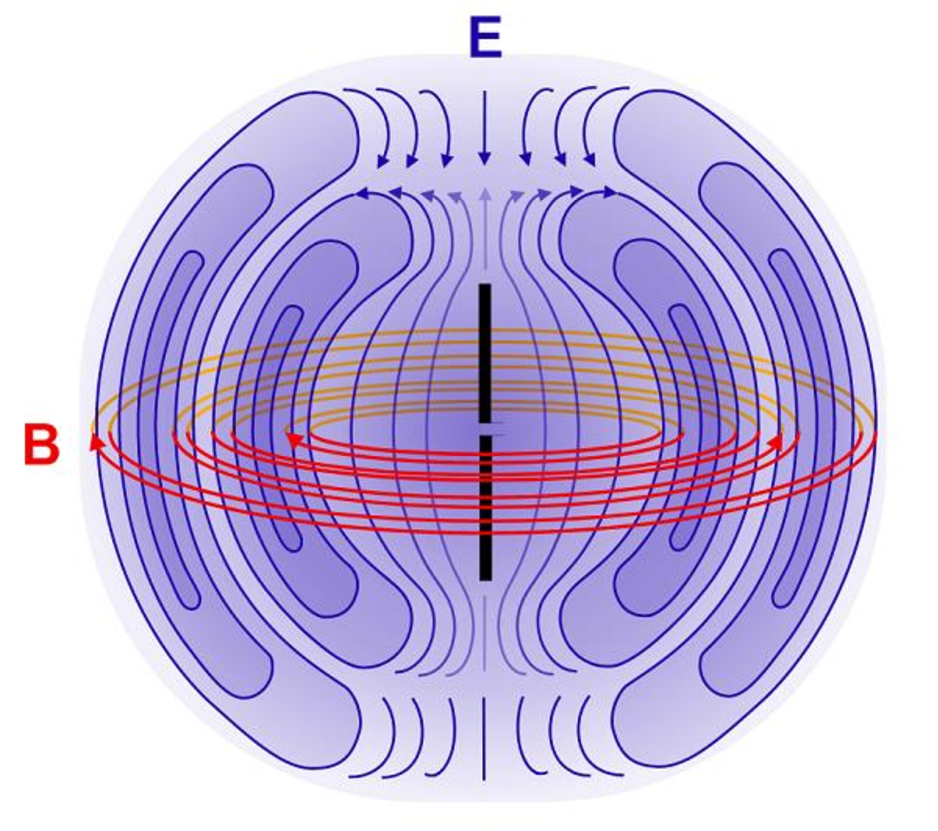
\includegraphics [width =0.5 \linewidth]{Apparatus-EM_field_antenna.pdf}
\end{center}
\caption[Electromagnetic field of a dipole antenna]{Electromagnetic field of a dipole antenna (image from \href{https://www.everythingrf.com/community/what-is-the-difference-between-a-monopole-and-dipole-antenna}{Everythingrf Website}). The near-field and far-field distribution are quite different as described in text.}  
\label{antenna_EM}
\end{figure}

% what previous one done, and what's the problem of it (done 2021-9-22 01:22:59)
Previously, we used a horn antenna for Rb MW transition at 6.8GHz. The distance between horn and atom is about 10-15 cm. The problem to put the antenna closer to the atom is its colossal size which could block the optical path, and its metallic body could disturb the strong magnetic field of a large Feshbach coil, causing a gradient on the atom. So the nearest position we can put is about 10 cm away from the atom, and the Rabi frequency of Rb $\ket{1,1}$ to $\ket{2,2}$ transition at 350 G (7.5 GHz) is less than 1 kHz with a 40 W power amplifier. The correspondents \(\pi/2\) pulse duration is about 250 $\mu$s which is too long for most of our experiments, such as high magnetic field image or too weak for dissociating the FR molecule. Thus, we need to upgrade it to enhance the Rabi frequency.

% full-loop antenna (done 2021-10-29 12:47:53)
\begin{figure}[htb]
\begin{center}
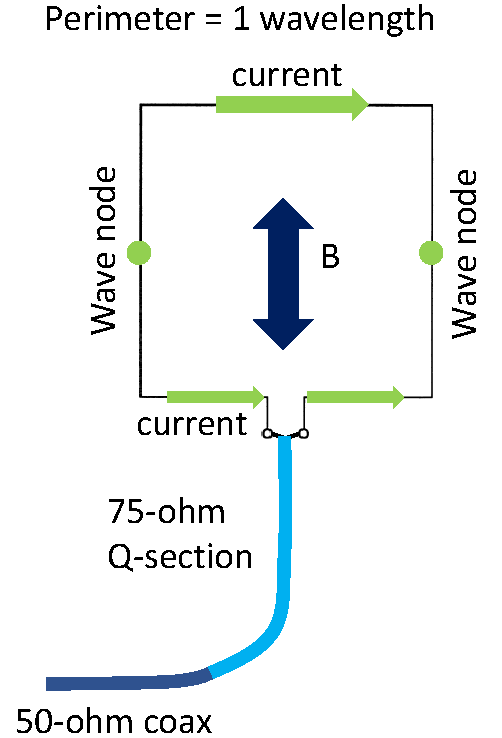
\includegraphics [width =0.5 \linewidth]{Apparatus_full_antenna.pdf}
\end{center}
\caption[Full loop antenna and Q-section for impedance matching]{Full loop antenna and Q-section for impedance matching. The parameter of the loop is set to be one wavelength of the emitting MW. The 75-ohm Q-section is for impedance matching.}  
\label{Apparatus_full_antenna}
\end{figure}

% How to improve? what is full-wave loop antenna? (done 2021-10-29 12:55:03)
So, a naive solution is to put the antenna as close to the cell as possible and try to shrink its size smaller and thinner. Therefore, the loop antenna will be a proper choice. A loop antenna is just a simple loop connected to the signal generator. However, for our case with frequencies at 2.6 GHz and 7.5 GHz, The wavelength is around several cm to tens of cm. This is comparable to our coil size, which could introduce a severe problem with impedance matching. A standard solution is making the perimeter of the loop antenna just a full wavelength, which is called the full-wave loop antenna as shown in Fig. \ref{Apparatus_full_antenna}. When the scale of the antenna is closed to wavelength, the distribution of radiation becomes quite different to those small-loop antennas. This can be explained by a simplified picture, as shown in Fig. \ref{Apparatus_full_antenna}. At the joint place, and directly opposite current changes with the largest amplitude, and there placed two nodes at the quarter wavelength place to the joint. However, the current almost has the same phase on the whole coil for a small loop antenna. Therefore, they have different radiation patterns.

% How the antenna works? (done 2021-10-29 13:00:50)
According to the near-field quasi-static EM field theory, the maximum radiation appears at \(\lambda/4\) away from the coil plane. Furthermore, the power at the centre of the coil is zero, which is different from the case of a small-loop coil. For our case with $f=2.6$GHz, the wavelength is about 12 cm. So, we place the coil 3 cm away from the atom to achieve the largest power. For the 7.5 GHz case for Rb MW in a high magnetic field, we set the perimeter of the loop to 4 cm. However, we cannot put the coil 1 cm away from the atom due to the distance limitation. Finally, by making the trade-off between the optical paths and MW power, we set the tiny coil at the side of the cell with a 45-degree angle and distance to atom about 3 cm. 

% Set-up and impedance matching (done 2021-9-22 02:35:26)
After preparing the coil, we set up the standard MW power amplifier circuit for it. Before the amplifier, we add a switch controlled by a TTL signal, and the signal generator is an SG-386. The critical point to increase the efficiency from power amplifier to the coil, i.e. \(\eta_{trans}\), we need carefully consider the impedance matching from the transmission wire to the loop coil. As shown in Fig. \ref{Apparatus_full_impedance}, we demonstrate several full-wave loop antennas with different shapes. They have different impedance; the ideal one is rectangular with an aspect ratio of 1:2, with 50 Ohm impedance. However, for our case with a round shape, we have the coil with 133 Ohm. Our transmission line and power amplifier are all 50 Ohm, so we need to match impedance. We use a balloon, i.e. a 75 Ohm transition line, to enhance the transmission rate. As shown in Fig. \ref{Apparatus_full_antenna}, the signal can be reflected at the boundary of two lines with different impedance. Boundaries of 50-to-75 and 75-to-133 offer two reflection waves. If we choose a proper length of the 75 Ohm line, we can cancel the reflection thanks to their superposition. 

% different shape and impedance (done 2021-10-29 13:12:09)
\begin{figure}[htb]
\begin{center}
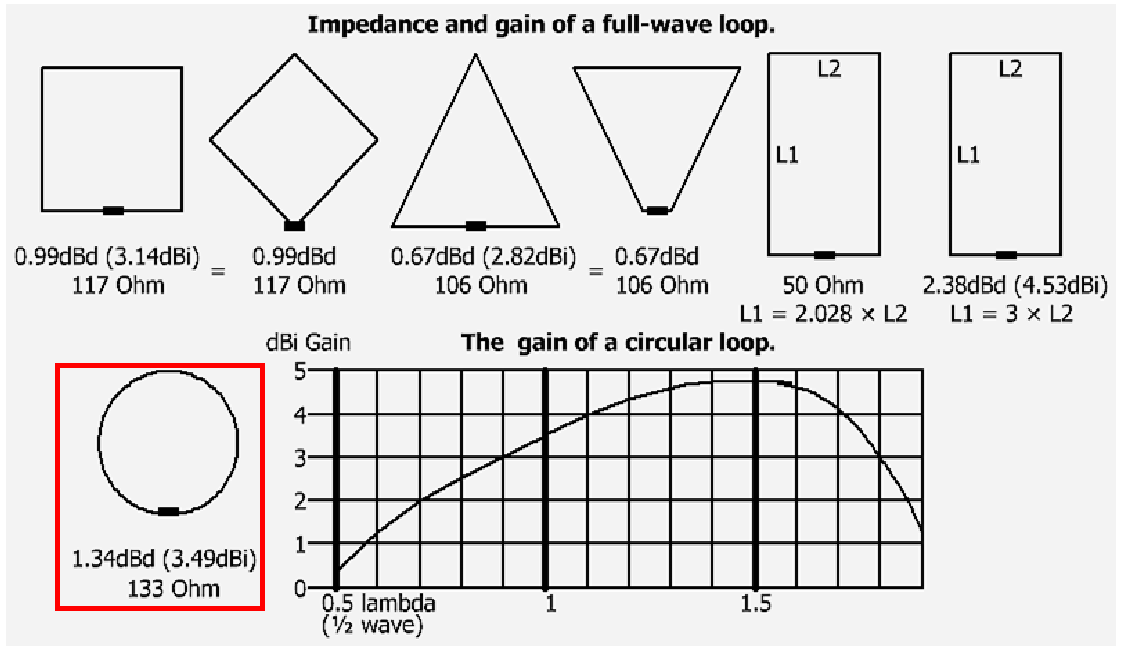
\includegraphics [width =0.8 \linewidth]{Apparatus_full_impedance.pdf}
\end{center}
\caption[Impedance of full-wave loop antenna with different shapes]{(image from \href{https://pa0fri.home.xs4all.nl/Ant/Quad/quadeng.htm}{pa0fri.home}) Impedance of full-wave loop antenna with different shapes. In our experiment, we use the round-shape to matching the optical path of MOT beam. In experiment in LH24C, the 1:2 rectangular is better since there is no need to do the impedance matching.}  
\label{Apparatus_full_impedance}
\end{figure}

% Test of the coil (done 2021-9-22 02:43:53)
Even though we know how long the q-section line should be, we still need to do the offline test for its performance because the length of several cm is too short to allow uncertainties from the imperfection of the coil's shape and impedance. These incomplete can cause the phase of reflection wave shifting and decline the effect of impedance matching. Therefore, we build a series of coils with different lengths of its q-section and measure its return loss rate by a directional coupler. As shown in Fig. \ref{SWR_measure_method}, we send the signal into the output port of a coupler, and the reflecting wave from the antenna (connecting on the input port of the coupler) will be coupled a small portion into the coupled port and detected by an analyser spectrum. By calculating the reflecting power and injection power, we plot the return loss rate as a function of the length of the q-section line in Fig. \ref{antenna_return_loss}. We find the period does coincident with the half of wavelength. There is a shift that could be attributed to the imperfection of the q-section line. By fitting with a sine function, we extract the period, shift and so on. Finally, We can now build the coil with the lowest return loss for covering our usage frequency.

% test the SWR by directional coupler (done 2021-10-29 13:06:48)
\begin{figure}[htb]
\begin{center}
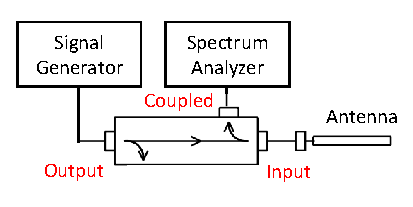
\includegraphics [width =0.7 \linewidth]{Apparatus-measure_SWR.pdf}
\end{center}
\caption[Test method of the return loss of the antenna]{Test the return loss of the antenna by a directional coupler. Noticed that the input signal is sent from the Output port of the coupler.}
\label{SWR_measure_method}
\end{figure}

% Online test (need more modification)
Finally, we put the coil onto the atom cell. First, we test the transmission rate of the coil online to make sure the impedance matching works well since the offline test with an environment open; however; however, the online environment is full of different metals around the coil, which could change the boundary condition and shift the impedance of the coil. So, we use the same method to test the transmission rate of the coil, as shown in Figure. The bandwidth is about xxx MHz. Then, we test the Atomic Rabi frequency to measure the final performance of the coil. We apply the MW pulse for Na at 350 G and get the Rabi frequency at different freq or detuning?. As shown in Figure, we test the saturation power and get a Rabi maximum of about 100kHz(check the number). This could allow us to make a pi pulse within 10 us which is enough for most cases such as optical pumping in the high field and MW spectroscopy.

% return loss measurement
\begin{figure}[htb]
\begin{center}
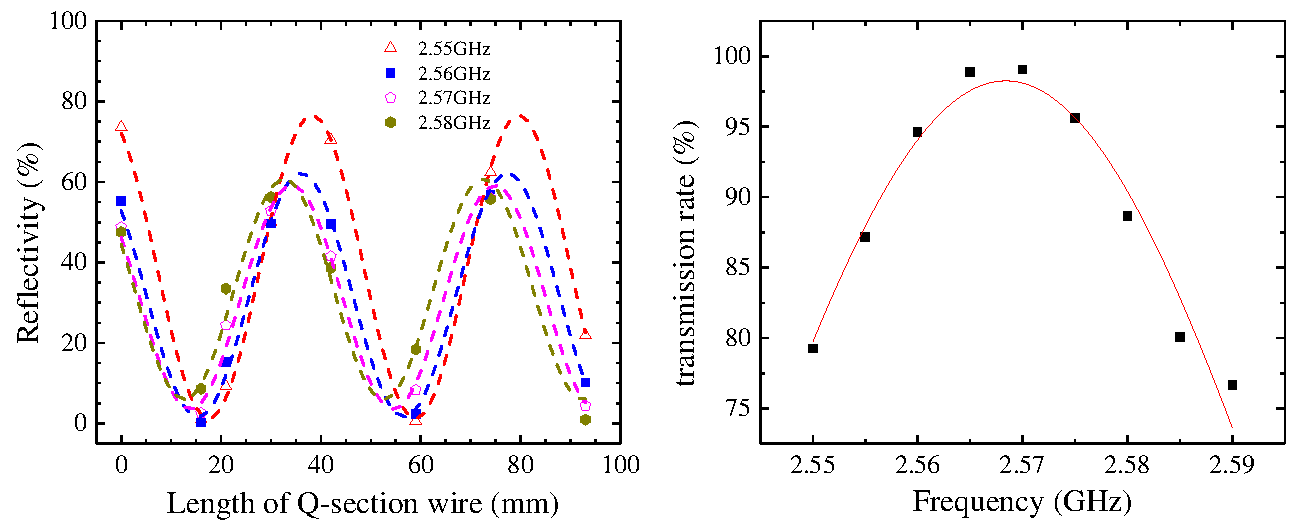
\includegraphics [width =0.95 \linewidth]{Apparatus-loop-antenna_retrun_loss.pdf}
\end{center}
\caption[Test of the return loss by changing the lengths of the Q-sections]{Test the return loss the full-wave loop antenna by changing the length of the Q-section line. Right side shows the band width test which provides a bandwidth of 67 MHz. }  
\label{antenna_return_loss}
\end{figure}

% about 6.8 7.5Ghz coil (done 2021-9-22 11:43:16)
After confirming that the 2.6 GHz coil does work, we built the 7.5 GHz coil, which could also increase the Rabi freq for Rb at high field. This one is similar to the Na coil with a parameter of 4 cm, which is relatively too small even to put it onto the science cell because it will block some part of the MOT beam. So, we choose to sacrifice power by arranging the coil on one edge of the cell, which increases the distance between the coil and atoms to about 3 cm. The best working distance for the 7.5 GHz coil is \(\lambda/4\), i.e. 1 cm, so for 3 cm distance, we get a power of about 1/3 compared to the maximum one. In order to pump atoms to the target state within tens $\mu$s, the required Rabi frequency needs about 10 kHz. Our online test shows a Rabi frequency of 10 kHz, allowing a 50 $\pi$-pulse for fast removing Rb atom from Feshbach molecules. Thanks to this new antenna, we can remove the horn antenna since the coil still works for 6.8 GHz with a transition rate of about \(10\%\), even its impedance matching point is 7.5 GHz. For typical MW evaporation, very little power is enough. Finally, removing the horn antenna leaves us much more space for future building optics layout.

% Rabi (done 2021-10-29 13:15:45)
\begin{figure}[htb]
\begin{center}
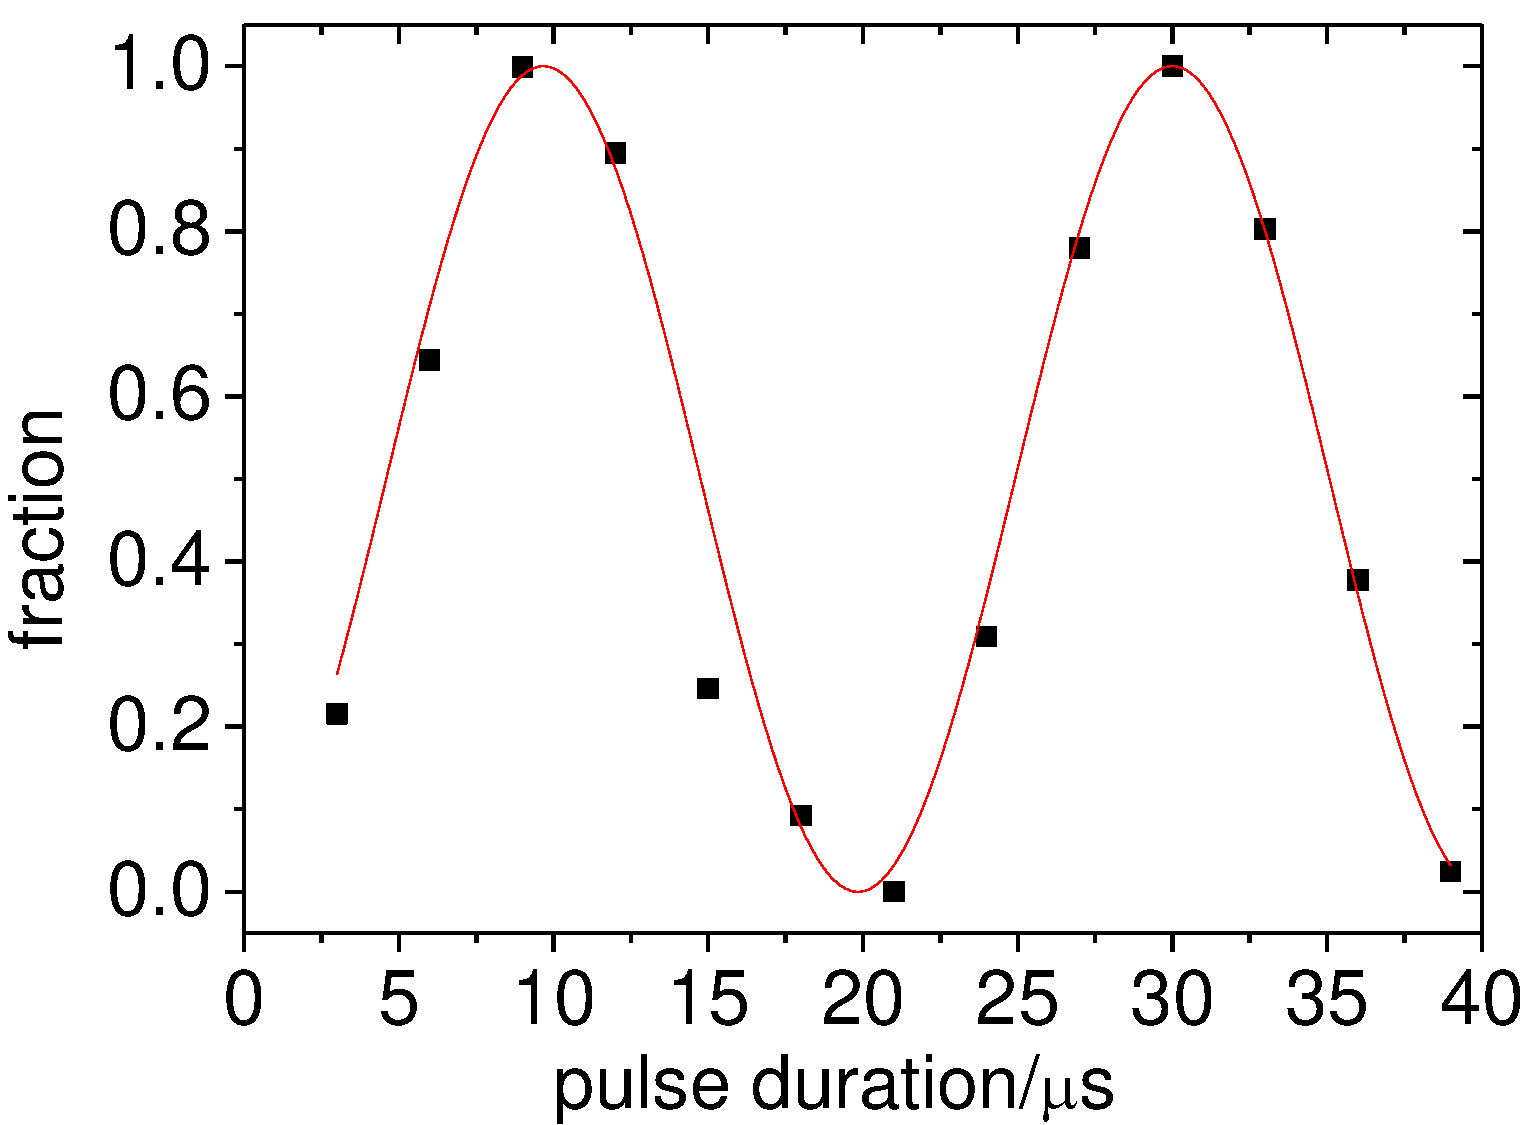
\includegraphics [width =0.7 \linewidth]{antenna_rabi.pdf}
\end{center}
\caption[Test Rabi oscillation of Na $\ket{1,1}$ to $\ket{2,2}$ under 350 Gauss magnetic field]{Test Rabi oscillation of Na $\ket{1,1}$ to $\ket{2,2}$ under 350 Gauss magnetic field. We can achieve a Rabi frequency of 50 kHz, which enable us pump atom to the target cycling transition within 10 $\mu$s.}  
\label{antenna_rabi}
\end{figure}

\chapterend